\chapter{ISR Simulation}
\label{chapter:stisrs}
\thispagestyle{myheadings}

% set this to the location of the figures for this chapter. it may
% also want to be ../Figures/2_Body/ or something. make sure that
% it has a trailing directory separator (i.e., '/')!
\graphicspath{{4_STISRS/Figures/}}

%%%%%%%%%%%%%%%%%%%%%%%%%%%%%%%%%%%%%%%%%%%%%%%%%%%%%%%%%%%%%%%%%%%%%%%%%

The following chapter will detail the methodology behind STISRS along with some processed examples. The first section will show how the synthetic data is created at complex voltage level. After which results of these simulations will be shown after the data has been processed as shown in Section \ref{section:isrproc}. The results will then be interpolated back to the original Cartesian space of the plasma parameters. 

\section{Simulation Methodology}

STISRS models space-time ambiguity using a coordinate transform and the pulse as a window along range while the statistical error is taken into account by creating complex shaped Gaussian noise. The simulation description begins with a description of construction of spectral filters designed to create the noise-like signal received in ISR experiments. This is followed by description of the process of creating complex receiver voltage data. 
\subsection{Creating Filters}

The simulator takes as input a discretized set of ionosphere state parameters in Cartesian coordinates which can vary in time.  This corresponds to the true field we will seek to reconstruct. The first step in the simulator is to create theoretical ISR spectra at each point from the prescribed parameters. For details on calculating these spectra from the intrinsic plasma parameters, see e.g. \cite{kudeki:milla:1} and \cite{kudeki:milla:2}. 

Once the spectra have been created, the simulator transforms the resulting values to a radar-centered spherical coordinate system. This coordinate change acts as a linear operator in spatial dimensions, and the spectra are accordingly weighted and averaged. The weighting in azimuth and elevation is determined by the antenna beam pattern, while the weighting in range (i.e. along beam) is simply just a binary test of whether the spectra are within the range gate. If there are no spectra within the range gate, a nearest neighbor rule is used which selects the closest point in Cartesian space. This method to create the spectra for each point is an acceptable approximation because spatial correlations between the electron density fluctuations will be on the order of the Debye length \cite{farley1969}, which is in nearly all practical cases significantly smaller than the beam width or range gate size. The algorithm implementing spatial sampling is shown in the simplified diagram in Figure \ref{fig:beamdia}.

\begin{figure}[!t]
\centering
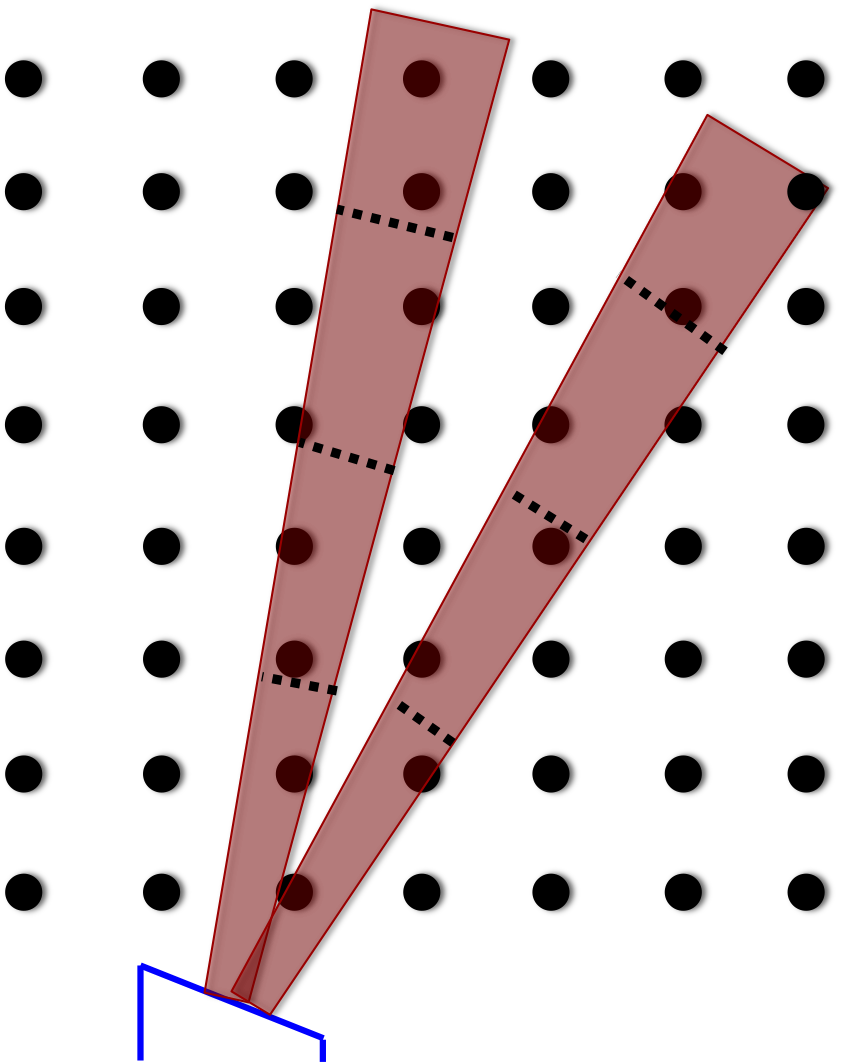
\includegraphics[width=2in]{beamsampling}
\caption{Each point is a from a discrete sampling of a Cartesian space. The beams are broken up into range gates, separated by the dotted lines, and the parameters at each point overlapping within these gates are averaged.}
\label{fig:beamdia}
\end{figure}
 
% Once the spectrum at the specific point in range and angle space has been determined, the filter $H_m(\omega)$, is created by simply taking the square root of the spectrum, $S_m(\omega | \: \bm{\theta})$,

% \begin{equation}
% \label{eq1}
% H_m(\omega) = \sqrt{S_m(\omega | \: \bm{\theta})}.
% \end{equation}

Once the spectrum for a given radar scattering volume has been determined, an appropriate spectral shaping filter is created. The method to create the filter given a desired spectrum or ACF can be done in a number of ways \cite{Kasdin:1995wi}. The current implementation in the simulator creates an infinite impulse response filter. The coefficients are determined using the ACF by solving the following set of equations,

\begin{equation}
\label{eq:filtereq}
\begin{bmatrix} R_m(0) & R_m(1)& \cdots & R_m(L-1) \\ R_m(L-1) & R_m(0)& \cdots & R_m(L-2)\\ \vdots & &\ddots  & \vdots \\  R_m(1) & R_m(2) & \cdots & R_m(0) \end{bmatrix} \left[ \begin{array}{c} a_1\\ a_2\\\vdots \\ a_L \end{array} \right]=\left[ \begin{array}{c} R_m(1) \\ R_m(2)\\ \vdots \\R_m(L) \end{array} \right]
\end{equation}

\noindent where $R_m(l)$ are the ACF values, $L$ is the desired length of the filter, and $ a_i$ are the set of filter coefficients. The filter then takes the form in the frequency domain as the following,

\begin{equation}
\label{eq:filtz}
H_m(z) = \frac{G}{1-\displaystyle \sum_{l=1}^{L} a_l z^{-l}}.
\end{equation}
\noindent The gain term $G$ is used to make sure the noise is the correct variance. This can be calculated as 

\begin{equation}
\label{eq:gainterm}
G=\sqrt{\displaystyle \sum_{l=0}^L -a_l R_m(l)},
\end{equation}

\noindent where $a_0=-1$.  This method has been used in similar ways in other contexts, e.g. the creation of vocoders for speech processing applications \cite{rabinerdigitalspeech}.
%\noindent The term $ \bm{\theta}$ refers to the plasma parameters needed to make the spectrum. This filter then is used to create the synthetic IQ data.

\subsection{Simulated Complex Voltage Creation}

The algorithm used to create sampled complex receiver voltages employs a complex white Gaussian noise (CWGN) process ("plant") that is spectrally shaped at its output using a time domain filter. As stated in the previous subsection, each point in space and time will have a separate noise plant and filter which is derived from the plasma and radar parameters parameters.  Figure \ref{fig:IQdiagram} presents a representative example. 

\begin{figure}[h!]
\centering
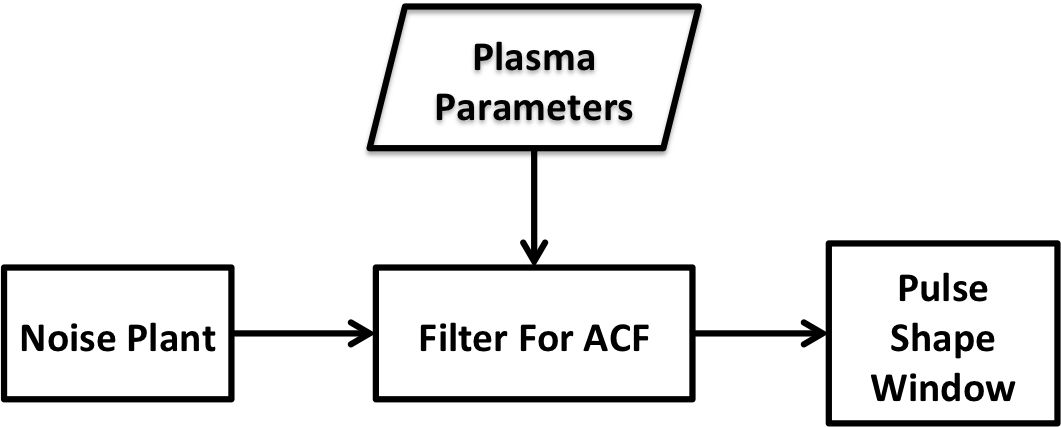
\includegraphics[width=4in]{diagrampart}
\caption{Diagram for complex receiver voltage simulator signal flow.}
\label{fig:IQdiagram}
\end{figure}

The creation of one set of complex receiver voltage data can be represented as the following  :   

\begin{equation}
\label{eq2}
y_m (k)= s(k)\left[h_m(k)*w(k)\right],
\end{equation}
 
\noindent where $s(k)$ is the overall transmitted pulse envelope, $h_m(k)$ is the time domain representation of the filter in Equation \ref{eq:filtz} and $w(k)\sim CN(0,\mathbf{I})$ or CWGN noise process. The pulse shape acts as a window, since the plasma will only reflect energy during the time it is illuminated by the radar signal. 
%The application of this filter is actually done in the frequency domain. This is possible because the Discrete Fourier Transform (DFT) of a vector of CWGN is also CWGN. The only difference is that there is a change in the variance, which is tied to the number of points used in the DFT \cite{kayvol1}. With this in mind Equation \ref{eq2} can be implemented as the following,

%\begin{equation}
%\label{eq:fftfilt}
%y_m (k)= s(k)\displaystyle \sum_{i=0}^{K-1}e^{j\omega_ik}\left[ \sqrt{S_m(\omega_i | \: \bm{\theta})}w(\omega_i)\right],
%\end{equation}
%
%\noindent where $\omega_i$ is the frequency variable, $w(\omega_i) \sim CN(0,\mathbf{I})$ and $K$ is the number of points used for the DFT \cite{michellnoisesim1981}.

\begin{figure}[!h]
\centering
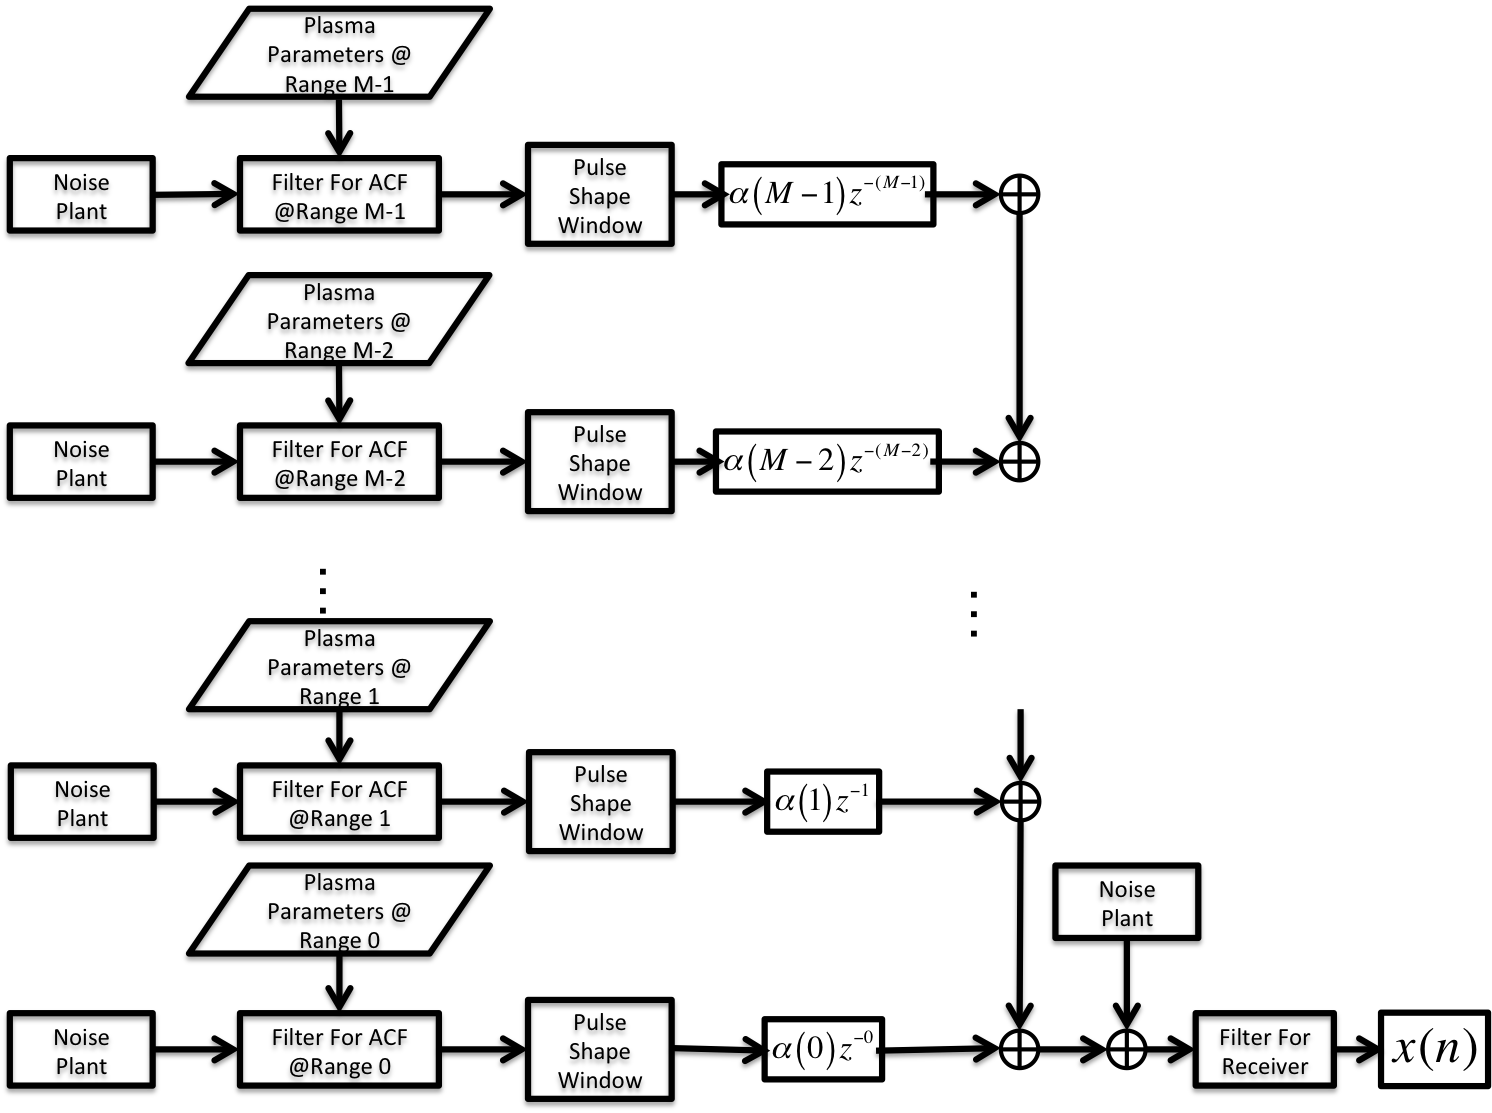
\includegraphics[width=7.0in]{diagram}
\caption{ISR simulation diagram.}
\label{fig:isrdiag}
\end{figure}


After the data for each range gate $y_m(k)$ is created, the received signal's power spectrum can be calculated from ISR plasma scattering theory as 

\begin{equation}
\label{eq3}
P_r = \frac{cG \lambda^2}{2(4\pi)^2}\frac{P_t }{R^2}\frac{\sigma_e N_e}{(1+k^2\lambda_D^2),(1+k^2\lambda_D^2 + T_r)},
\end{equation}
 
 \noindent where $P_r$ is the power received in Watts (W), $k$ is the wavenumber of the radar in meters (m), $c$ is the speed of light in m/s, $G$ is the gain of the antenna, $P_t$ is the power of the transmitter in W, $\sigma_e$ is the electron radar cross section in $m^2$,  $\lambda_D$ is the Debye length in m, $N_e$ is the electron density in m$^{-3}$and $T_r$ is the electron to ion temperature ratio.
  
The received signal power calculated at each range gate using equation~\ref{eq3} is used as a scaling constant for each $y_m(k)$ series.  Finally, a delayed and summed operator yields a model of the received radar scatter signal:
 
\begin{equation}
\label{eq4}
x(n) = \displaystyle\sum\limits_{m =0}^{M-1} \alpha(m)y_m(n-m),
\end{equation}

\noindent where $\alpha(m) = \sqrt{P_r(m)}/\widehat{\sigma_y}$ and $\widehat{\sigma_y}$ is the estimate of the standard deviation of $y_m(k)$. Lastly, to model total noise from the radar system and environment, an additive CWGN process is included, creating the final simulated complex receiver voltage sequence

\begin{equation}
\label{eq:addnoise}
x_f(n) = x(n) +\sqrt{\frac{k_bT_{sys}B}{2}} w(n), \quad w(k)\sim CN(0,\mathbf{I})
\end{equation}

\noindent where $k_b$ is Boltzmann's constant, $T_{sys}$ is the system temperature and $B$ is the system bandwidth.
A full diagram of the model can be seen in Figure \ref{fig:isrdiag}.

\section{Simulation Examples}
The framework for STISRS allows exploration of a number of aspects of ISR processing. Within the scope of this article, we will focus on three application examples.

The first example demonstrates how the simulator can be used for Monte Carlo estimates of ISR spectra. In this case, we hold all of the plasma parameters constant and determine how the distribution of the measured parameters evolve. The next example uses a simple altitude distribution of ionospheric plasma parameters to show the impact of the forward model of the ISR on a basic measurement of electron density. This is intended to illustrate that basic ambiguities inherent in ISR measurements can give the appearance of a change in morphology of the plasma phenomena when none truly exists. Finally, the output of a fully consistent multi-fluid ionosphere model is used as input to the ISR simulator to show a use case relevant to experiment planning. This case illustrates an inherent tradeoff in experiment construction between reducing statistical fluctuations in the measurement and increasing distortion in the final reconstruction.

\subsection{Monte Carlo Example}

It is often necessary to get a large number of sensor measurements for a statistical study or perhaps create a training data set for a pattern recognition algorithm. This can require large amount of work by the researcher to search and classify the different data. Fortunately there may be cases where one could use STISRS to create some synthetic data instead.

%\pcom{Very awkward and verbose; rewrite}{It is necessary to understand the statistics from the sensors used in scientific studies. In order to do this a large number of measurements must be taken with the sensor. There are issues with this approach in that the inputs can not be controlled so along with any random variation that may be found in the sensor the random variation of the measured process will be included and must be taken into account during the analysis of the data. With the simulator the statistical fluctuations from only the measurement mechanism only can be studied and thus reducing the uncertainty of the measurements.}

For this example we show how distributions of plasma parameter measurements change as more pulses are averaged. To do this we created a field of constant plasma parameters typical of the high latitude ionosphere at around 250 km, and performed a Monte Carlo type simulated statistical experiment using a number of independent realizations. We use the parameters for the Poker Flat AMISR system for this simulation along with the plasma parameter listed in Table \ref{tb:param1}. For a number of independent radar pulse counts $J$, we used 4,600 realizations of the statistical ISR measurement process in each case to create statistical distributions of measured parameter values. The distributions can be seen in Figure \ref{fig:statshistall} which show distributions where 200, 500 and 1000 pulses are used respectively. For a given pulse count $J$, the plasma parameters have a Gaussian-like distribution. Furthermore, as expected the distribution narrows as the number of pulses $J$ is increased.  

\begin{table}[!t]
\centering
\caption{Simulation parameters.}
\label{tb:param1}
\begin{tabular}{ll}
Species & O+ e-\\
$N_e$    & $1\times 10^{11}$ \\
$T_e$      & $2100^o$ K   \\
$T_i$      & $1100^o$ K \\
$V_i$      & $0$ m/s
\end{tabular}
\end{table}

\begin{figure}[!t]
\centering
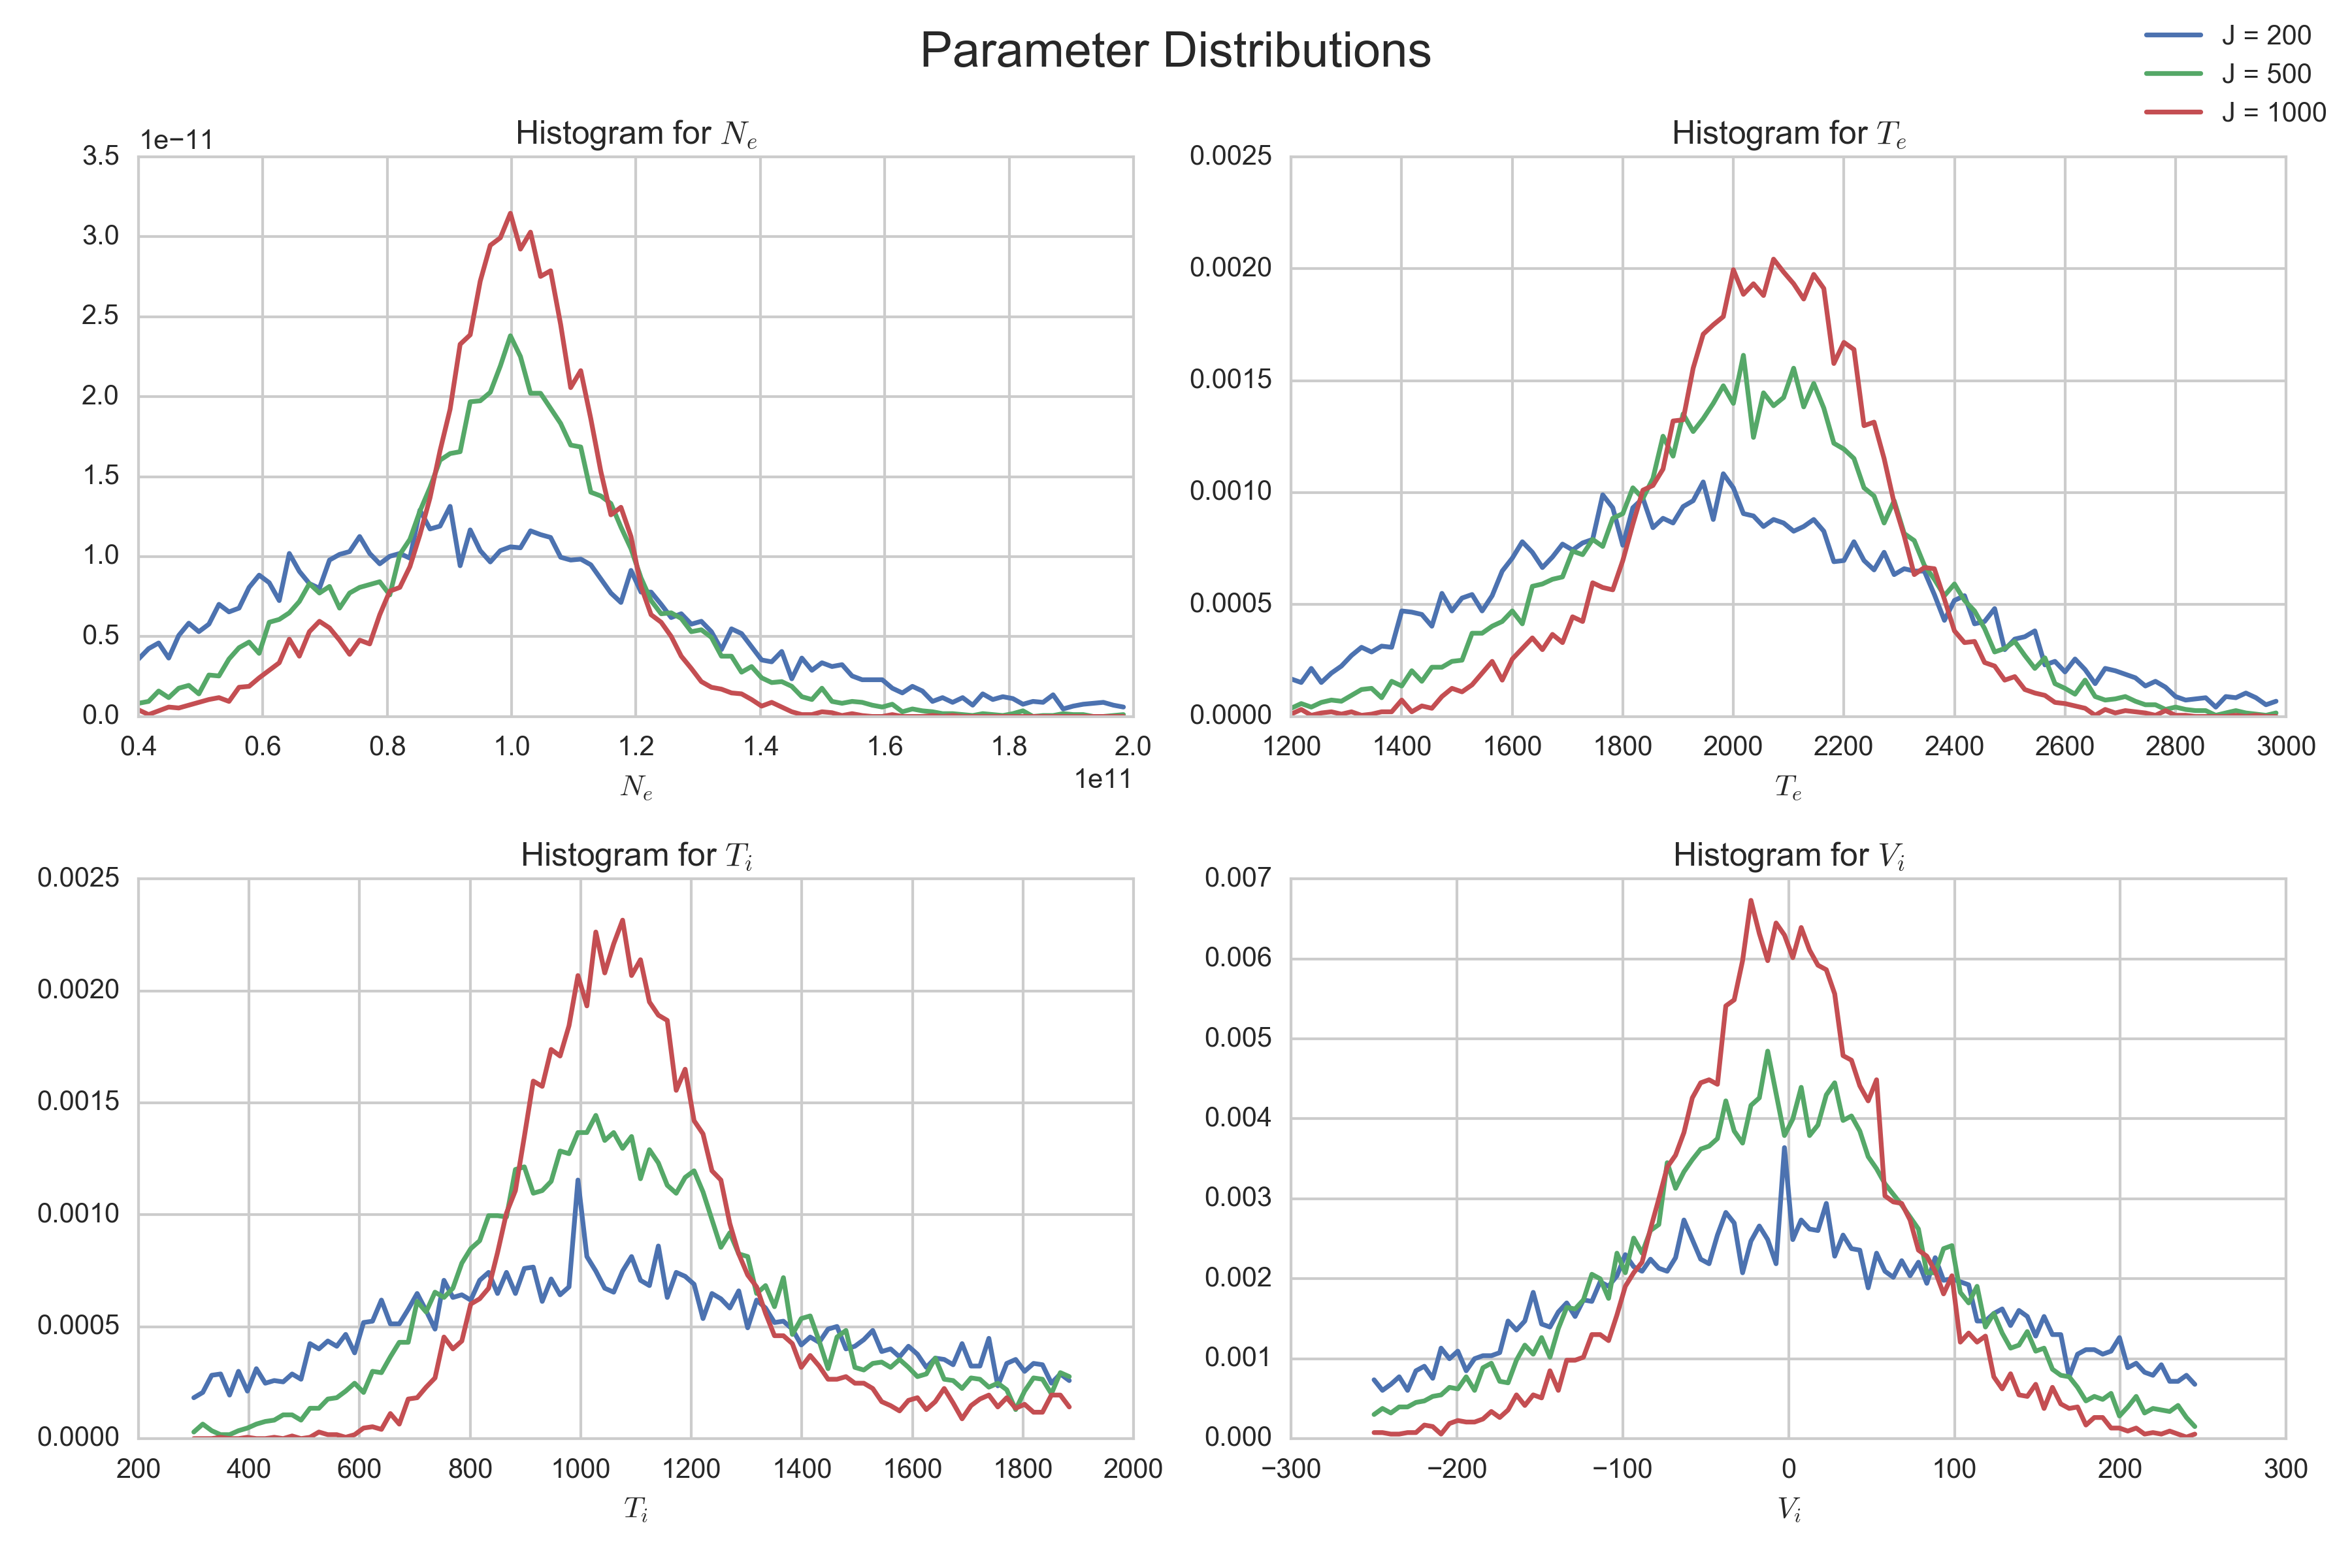
\includegraphics[width=5in]{datahist}
\caption{Normalized histograms of fitted plasma measurements from cases with 200, 500 and 1000 pulses integrated. These are estimates of probability density functions for each of the plasma parameters measurements given the values in Table \ref{tb:param1}.}
\label{fig:statshistall}
\end{figure}

One utility of being able to create a large number of samples of fitted parameters is seen in error analysis. ISR measurements need to have estimates of the errors, and accuracy of the estimates of these errors can be explored using STISRS. Using case seen in Figure \ref{fig:statshistall} with 1000 pulses we can compare the actual distribution of parameter values. Figure \ref{fig:statshistsingle} shows gives a comparison of these two different models using, one using the sample variance calculated from each parameter and the average estimate of the error, as the variance and average value for the mean. This example shows that the parameter distributions can be well represented by a Gaussian function but that the error estimated from the fit, may not give a completely accurate representation of variance of these parameters. 

\begin{figure}[!t]
\centering
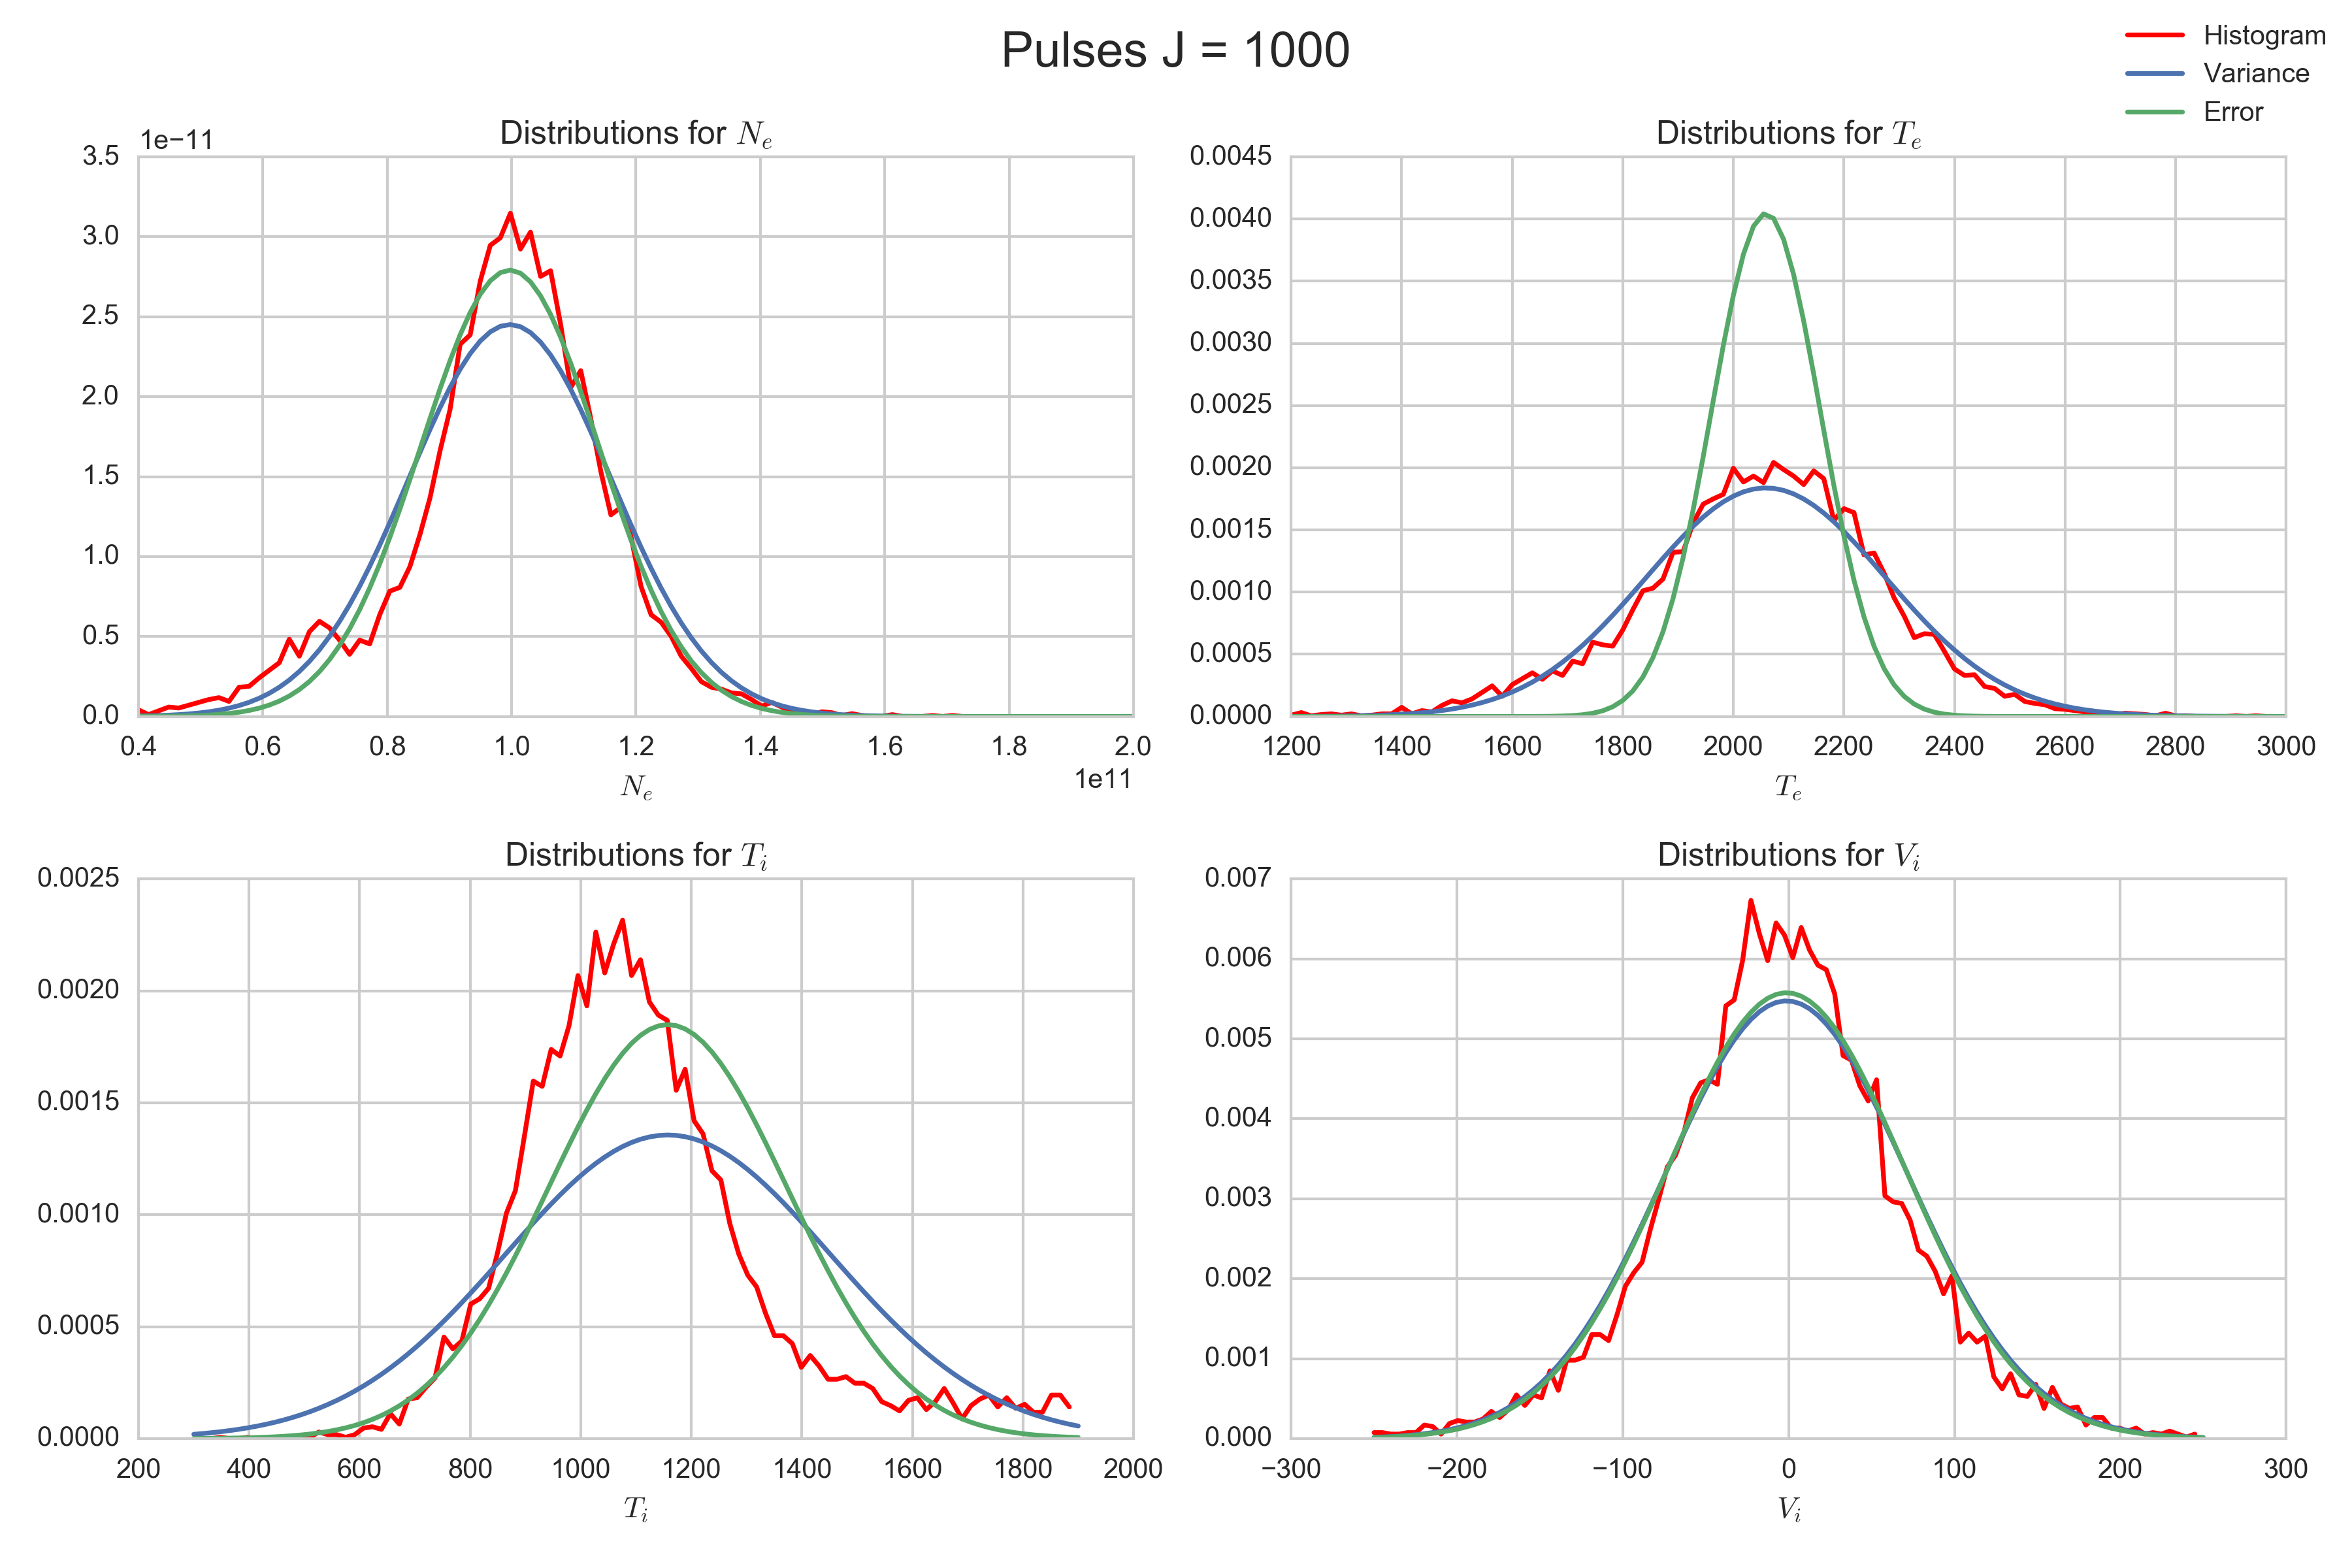
\includegraphics[width=5in]{histsingle}
\caption{Distributions of fitted plasma measurements from cases with 1000 pulses integrated. The red curve shows the actual distribution derived from a histogram of 4600 measurements. The blue curve is a Normal distribution using the MSE from the measurements as the variance and the average parameter value as the mean.  The green curve is a Normal distribution using the average estimate of error squared that comes with the parameter measurement as the variance and the average parameter value as the mean.}
\label{fig:statshistsingle}
\end{figure}


STISRS can useful for identifying situations where assumptions in the parameter fitting break down. For example, a number of studies have explored the case where ISR parameter measurements and spectra show evidence of non-Maxwellian plasma behavior \cite{Akbari:2012dz,Akbari:2015fv}. Future studies using the simulator could help create a training set that can be used with a pattern recognition algorithm to identify cases where normal fitting procedures may be incorrect.

\subsection{Electron Density Measurement}
An important aspect of experiment design is determining the observability of plasma phenomena with ISR. The simulator can be used to help understand the trade space accompanying each experiment. With this in mind, we use a simple two dimensional spatial field of ionospheric parameters as a demonstration case study. An all-O$^+$ ionosphere is created with a background electron density that follows a Chapman function with $1\times10^{11}$ m$^{-3}$ as the peak value and a constant electron and ion temperatures of 2000 $^\circ$K and 1500 $^\circ$K respectively. The background electron density can be seen in left panel of  Figure \ref{fig:background1}.

\begin{figure}[!t]
\centering
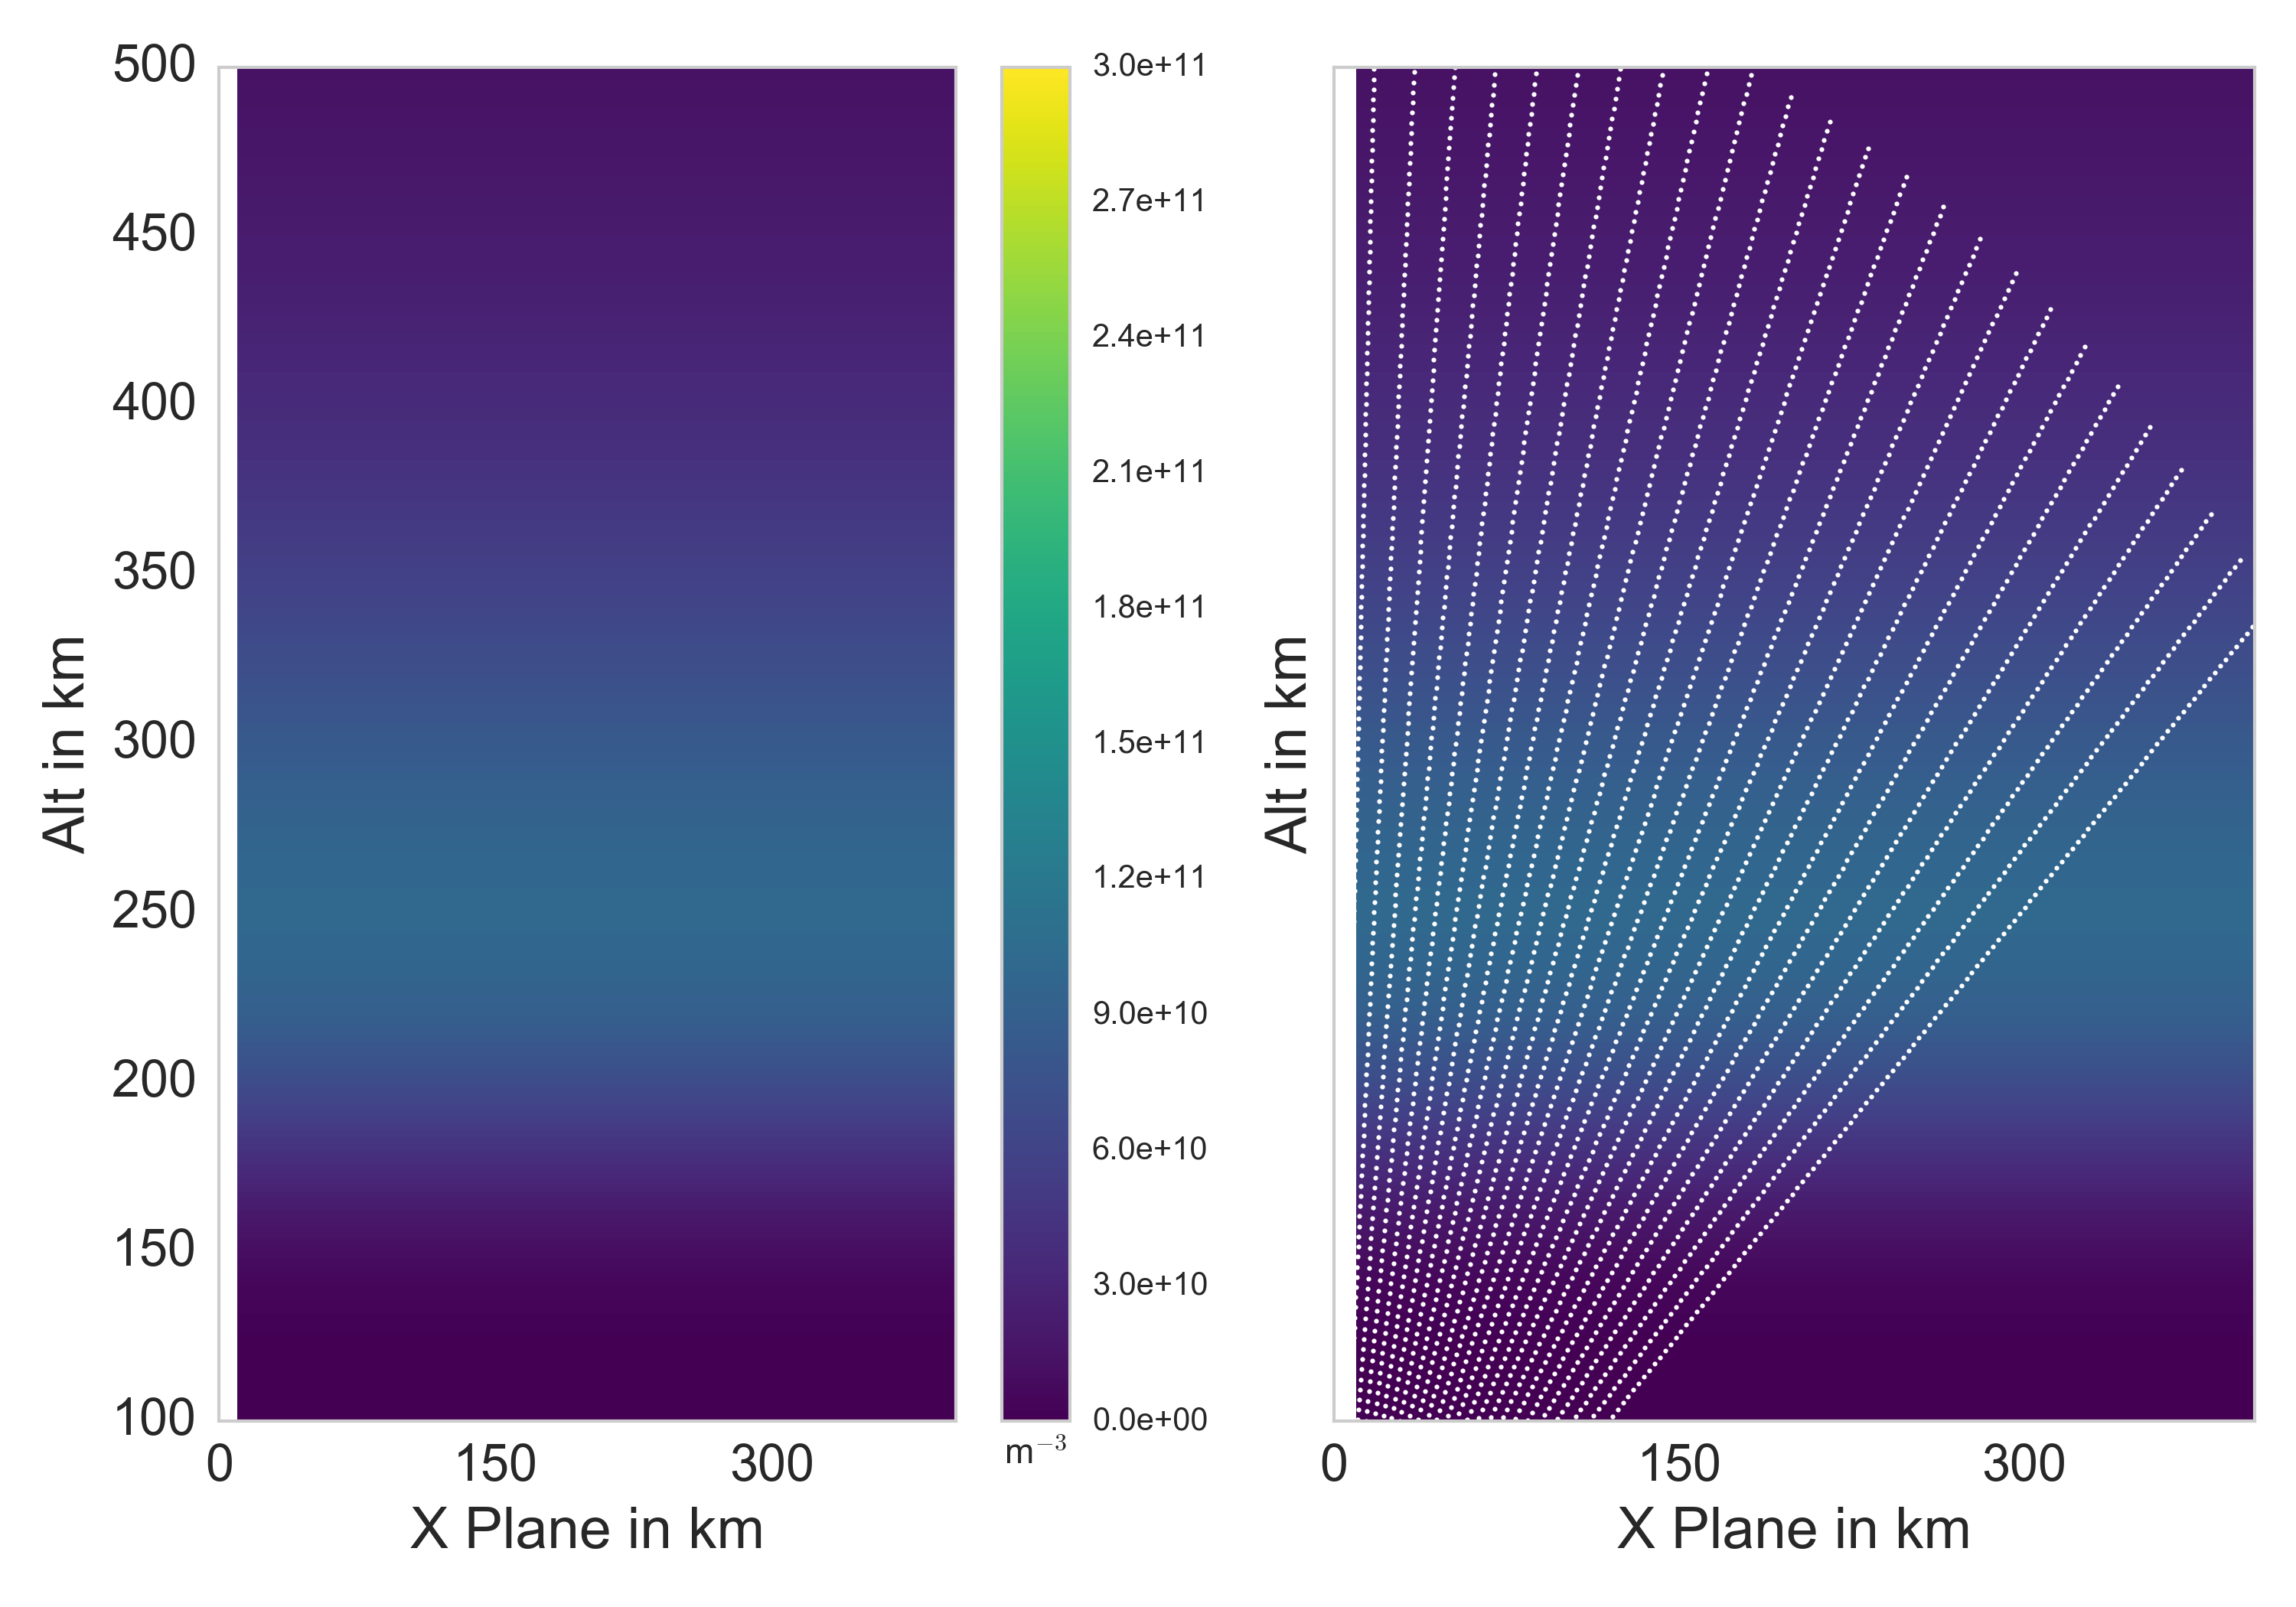
\includegraphics[width=4in]{backgroundandsamp}
\caption{Contour of background $N_e$ for simulations and the spatial sampling pattern}
\label{fig:background1}
\end{figure}

%For these simulations we want to show how ambiguities could arise when trying to image just simple electron density enhancements with the beam pattern shown in the right panel of Figure \ref{fig:background1},
For these simulations we explore how a thin density enhancement is resolved with a radar beam pattern shown in the right panel of Figure \ref{fig:background1}, where each dot is a range gate in one of the 25 beams used. This thin density enhancement is 2 km in width and enhances the density by 5 times the background at its altitude. The enhancement is at the resolution limit of the original Cartesian grid, a delta function in the x direction. The results of a single realization of our simulation are seen in Figure \ref{fig:stationaryall} using a 15 second and 60 second integration time, 60 and 240 pulses per position respectively. The different integration times show that, although the enhancement is blurred, the variance of the measurement can impact the quality of the reconstruction because of the inherent noise quality of the signal. The expected errors for both of the reconstructions can be seen in \ref{fig:errorstationaryall}. As expected the estimated errors show the uncertainties for the case with less pulses to be larger. 

Because we know the input parameters we can do a quick comparison using the root mean squared error (RMSE) for each case. If we comparing the RMSE between the 15 and 60 second integration cases we find that the ratio between the two is approximately 5.40. The expect RMSE ratio between the two should be about 2 because the variance of the ACFs scales as $1/\sqrt{J}$, where $J$ is the number of pulses. If we instead median instead of a mean operator in the error calculation this ratio becomes 1.55 which is some what more in line with what is expected.

\begin{figure}[!t]
\centering
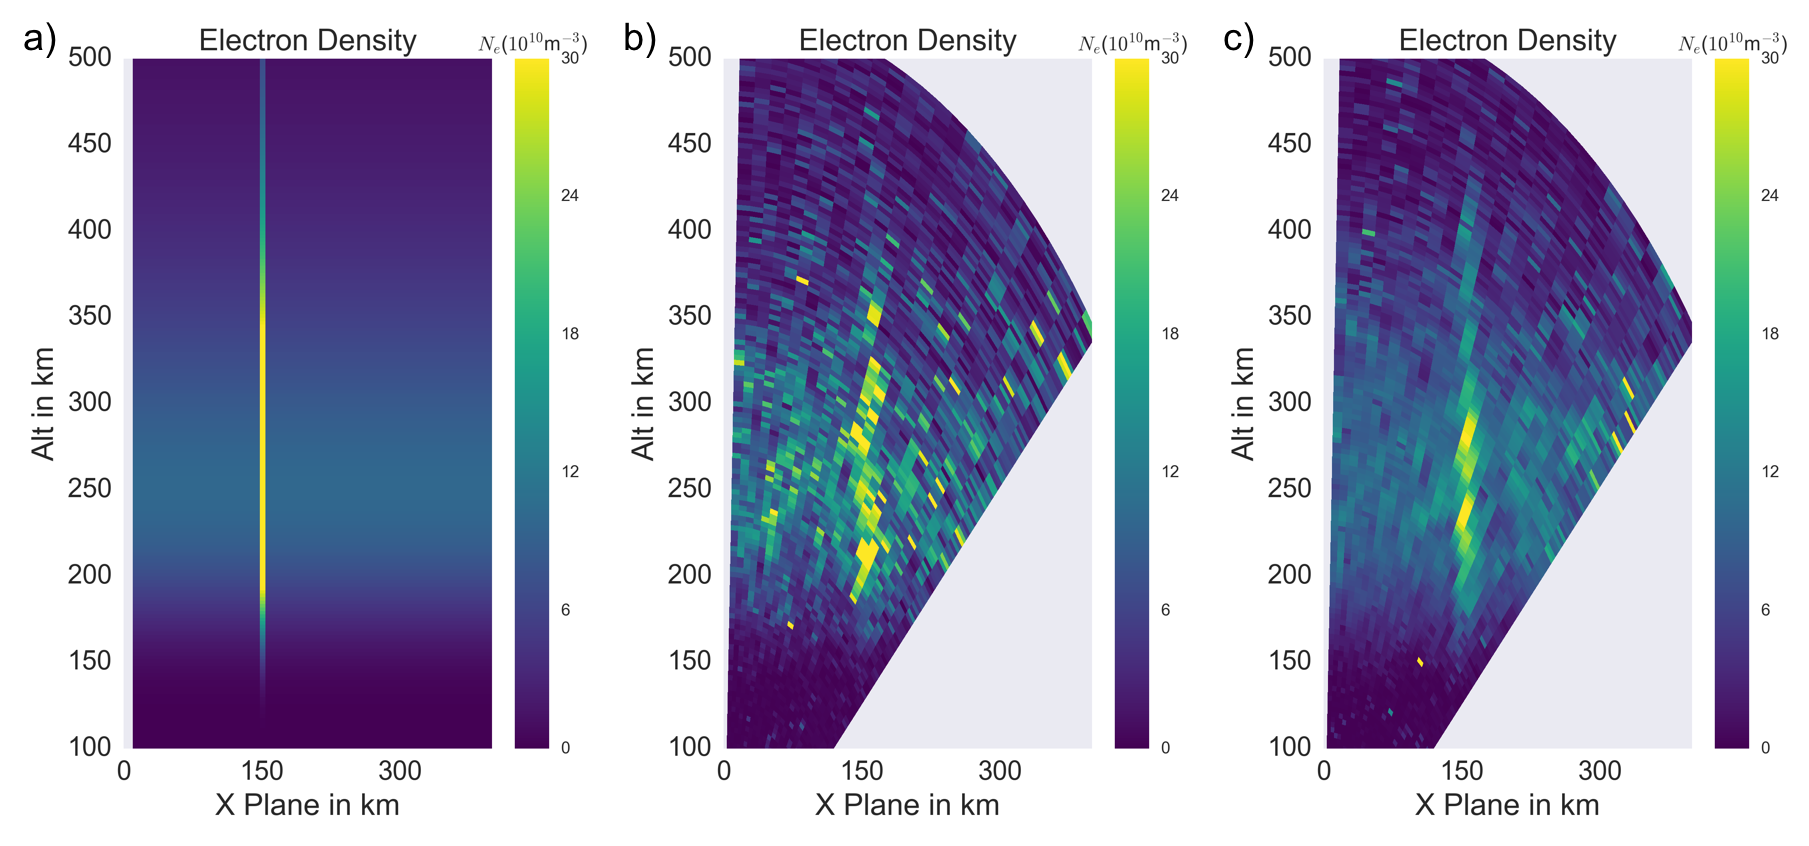
\includegraphics[width=6in]{stationary}
\caption{Results of stationary enhancement simulation. a) Input $N_e$. b) Output of simulator with 15 second integration. c) Output of simulator with 60 second integration.}
\label{fig:stationaryall}
\end{figure}

\begin{figure}[!t]
\centering
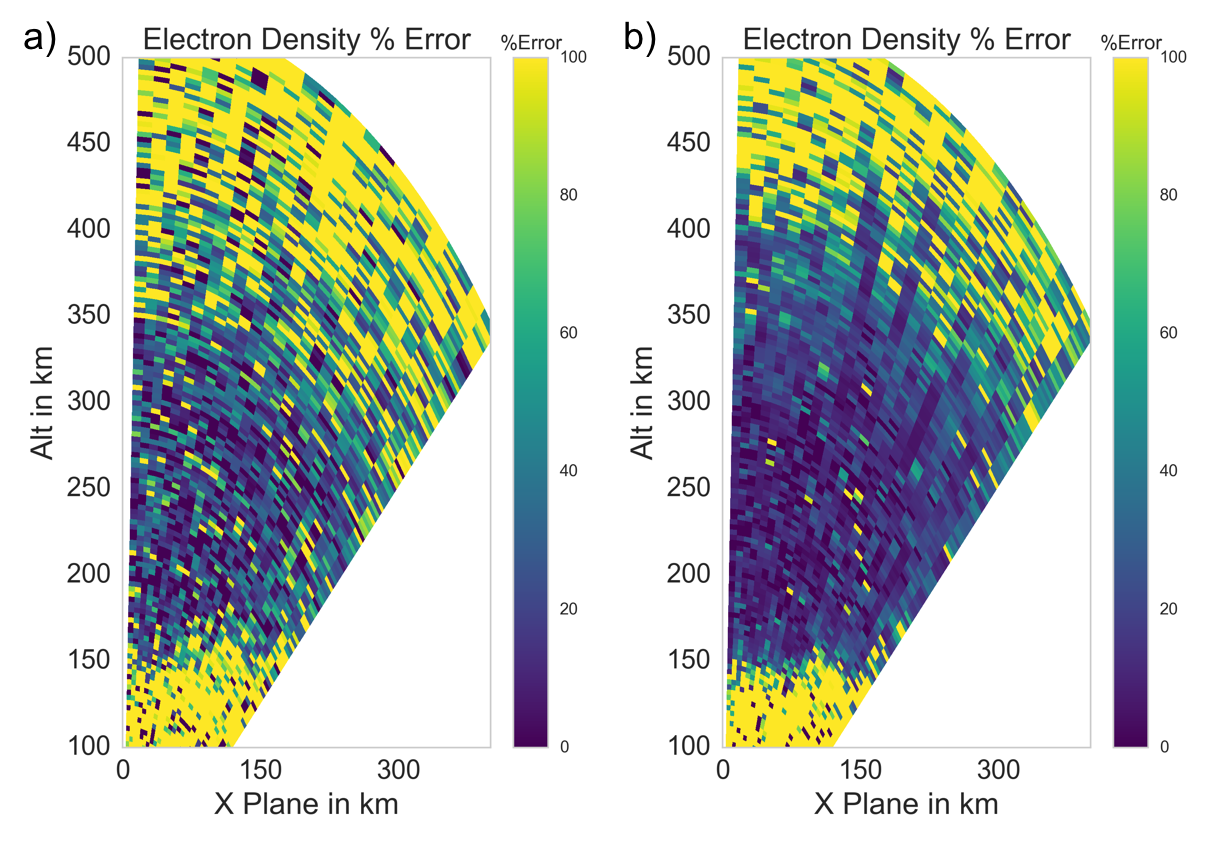
\includegraphics[width=4in]{Errorstationary}
\caption{Standard deviations from Figure \ref{fig:stationaryall}. a)  Estimate from fit for 15 second integration example. b) Estimate from fit for 60 second integration example.}
\label{fig:errorstationaryall}
\end{figure}

The blurring effect seen in this case study is not constant throughout the space due to the way the radar samples the space. This is illustrated in Figures \ref{fig:moving10mins} and \ref{fig:moving14mins}, where as the enhancement moves through the scene, its apparent size is affected by the orientation of the radar beams. As the enhancement becomes parallel to the radar beams then the shape in the reconstruction becomes smaller along the x-axis, as the range ambiguity is much larger than the cross range ambiguity from the beam pattern.

\begin{figure}[!t]
\centering
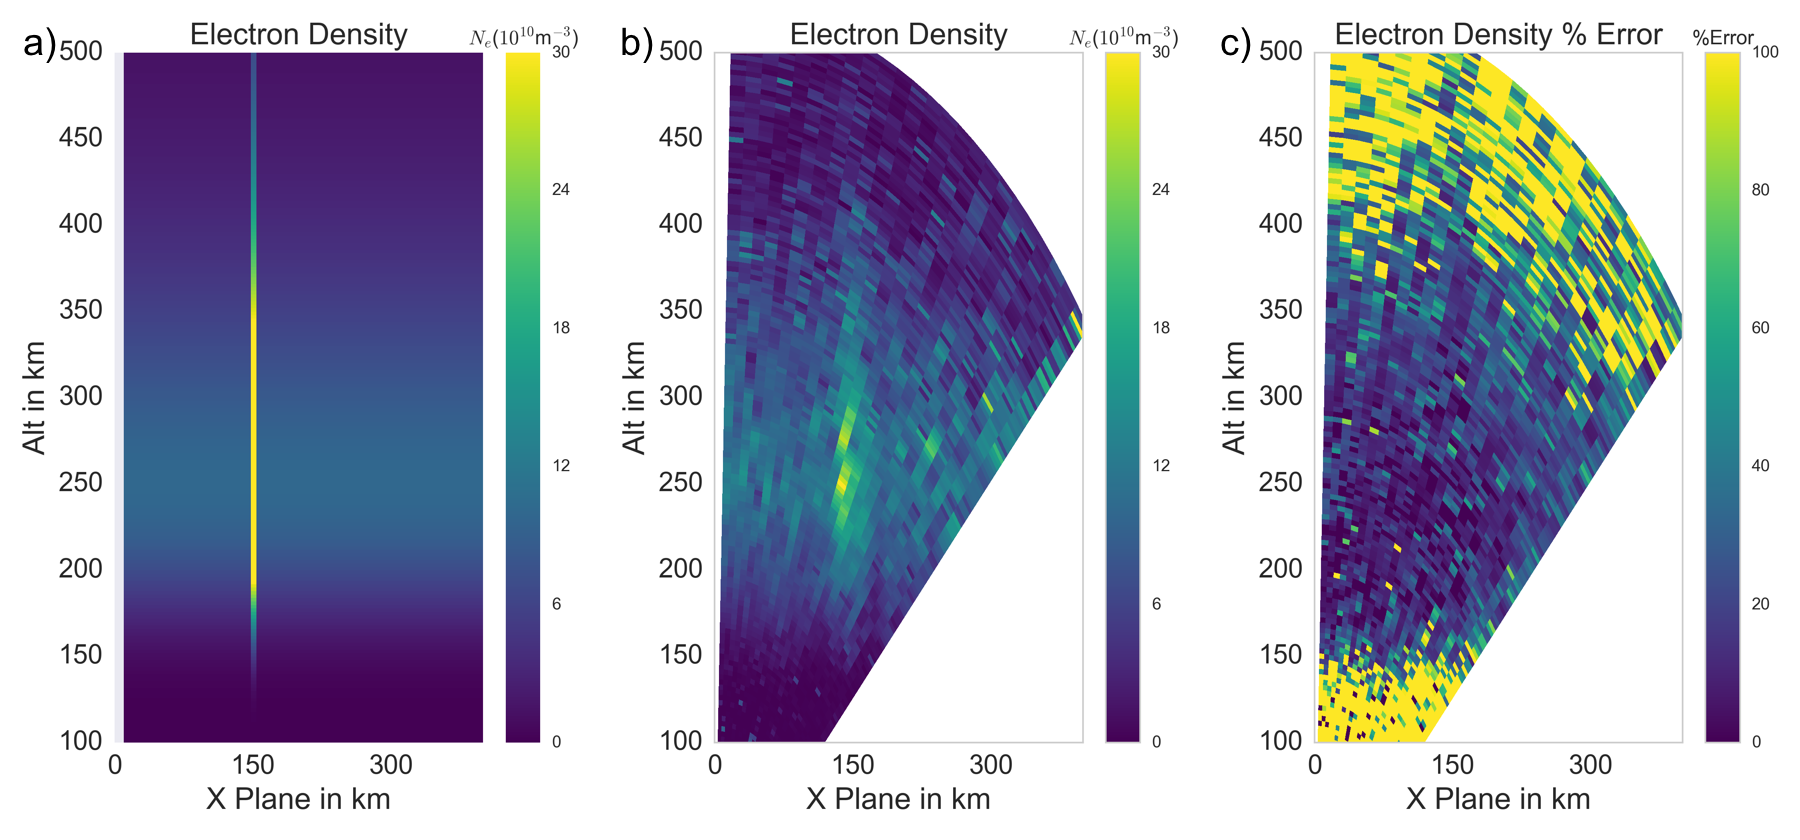
\includegraphics[width=6in]{moving6mins}
\caption{Results of moving enhancement simulation at 600 seconds. a) Input $N_e$. b) Output of simulator with 60 second integration. c) Estimated errors from fit.}
\label{fig:moving10mins}
\end{figure}


\begin{figure}[!t]
\centering
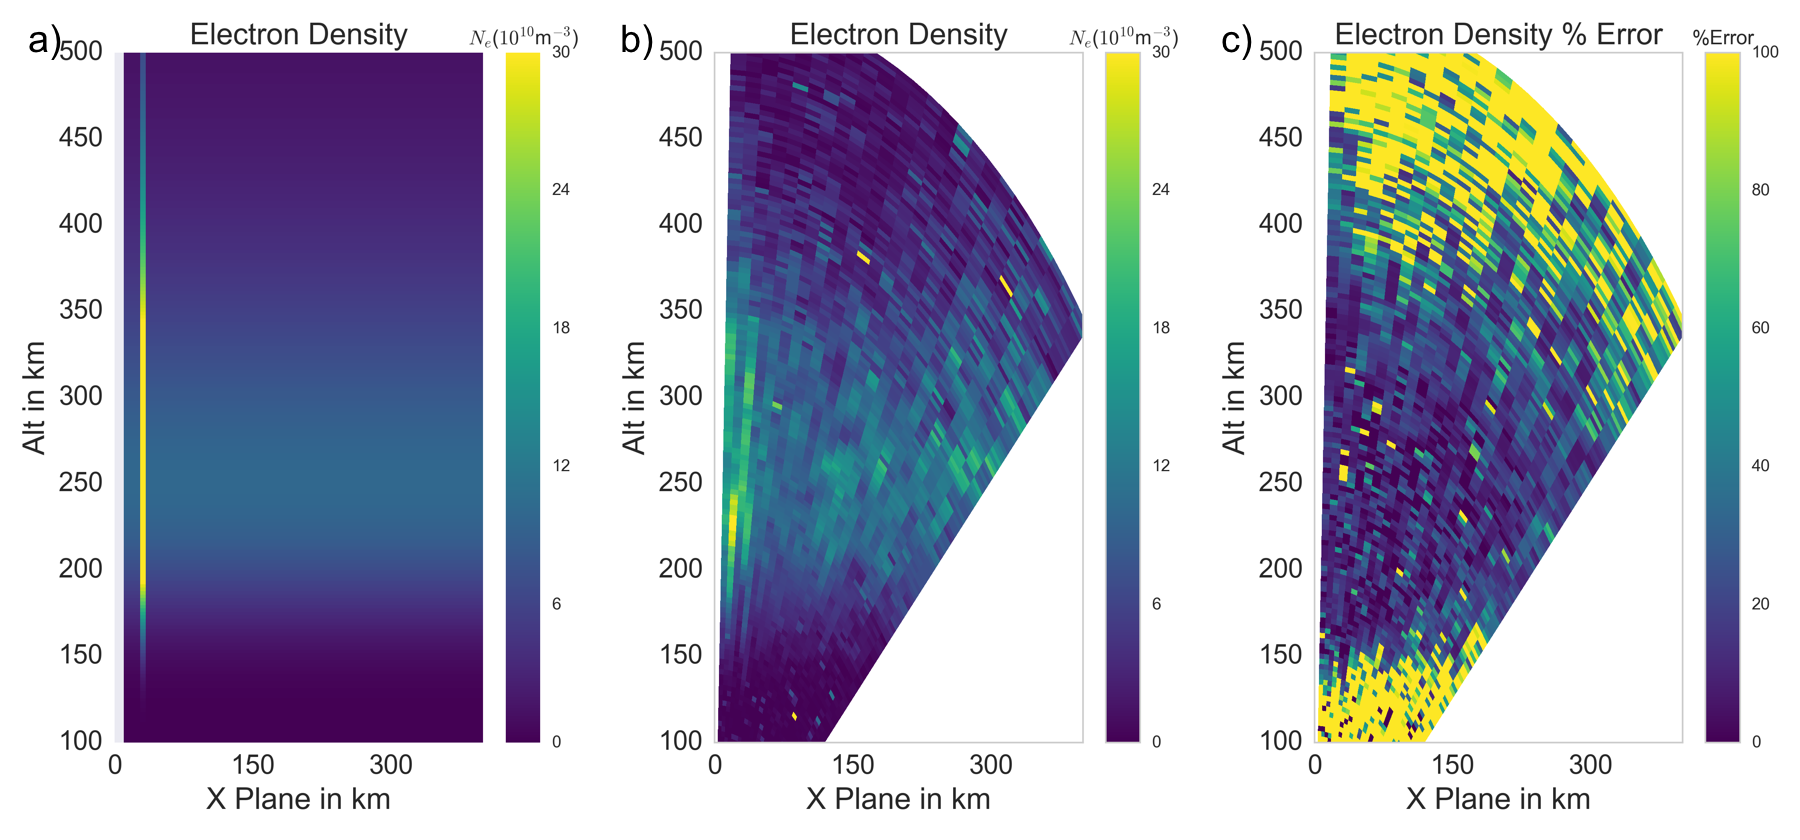
\includegraphics[width=6in]{moving14mins}
\caption{Results of moving enhancement simulation at 840 seconds. a) Input $N_e$. b) Output of simulator with 60 second integration. c) Estimated errors from fit.}
\label{fig:moving14mins}
\end{figure}

This change in the shape of the enhancement can give the impression that its morphology has developed as it was moving through the field of view of the radar. This could lead to an incorrect interpretation of the physical process taking place. Thus one must be careful when analyzing these sorts of reconstructions.

Lastly, for this type of simulation, we show an example to demonstrate the situation where a set of two different input parameters can yield qualitatively similar results. For these cases we create electron density enhancements similar in size as what is seen in \cite{Semeter:2005fo} from a poleward boundary intensification event. The sizes of these enhancement are 10 km width and 18 km width. The enhancement in the 10 km width example is 6 times higher than the background while the 18 km width enhancement is 3 times higher than the background.

The input electron density, the fitted electron density and the expected error for the 10 km enhancement can be seen in Figure \ref{fig:moving10all}. The same images for the 18 km wide case can be seen in Figure \ref{fig:moving18all}. Both cases show that electron density enhancements are well above the expected errors. The fitted electron density for 10 km enhancement the 18 km enhancement show nearly identical results. This simple example demonstrates the possibility to create a non-unique solution in ISR. But it also shows a utility for STISRS in that it can be used to determine if an experiment set up will lead to ambiguous results between two different sets of phenomena. 

\begin{figure}[!t]
\centering
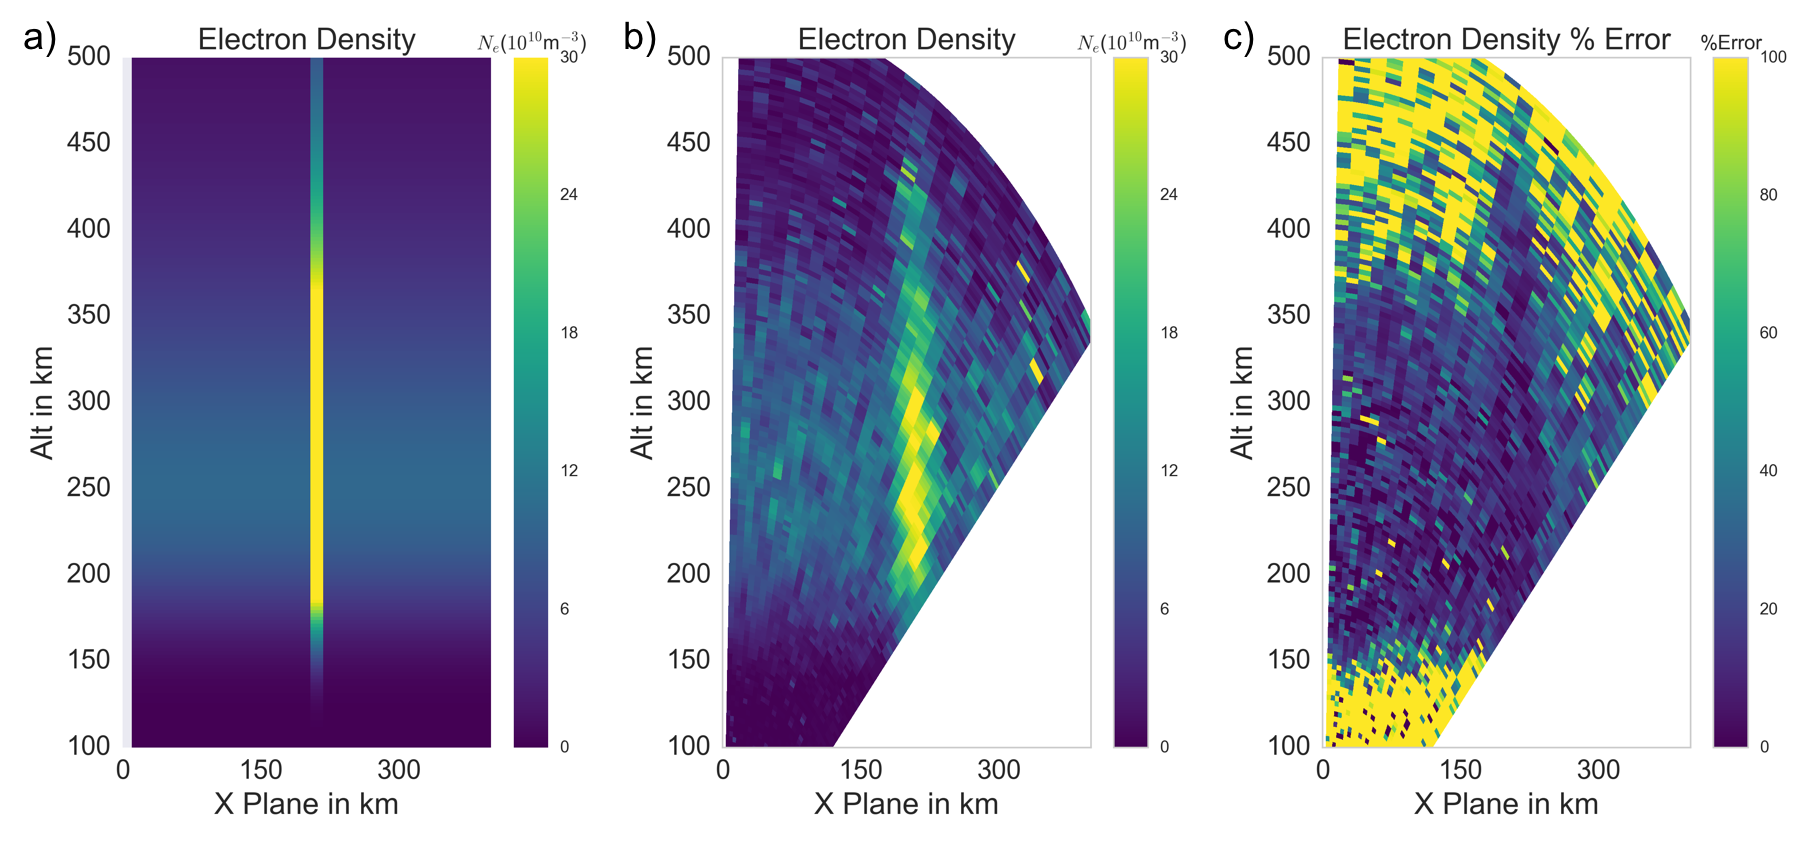
\includegraphics[width=6in]{moving10kminouterr}
\caption{10 km wide enhancement moving simulation at 480 seconds. a) Input $N_e$. a)  b) Fitted $N_e$ with 60 second integration. c) Estimated error from fit.}
\label{fig:moving10all}
\end{figure}

\begin{figure}[!t]
\centering
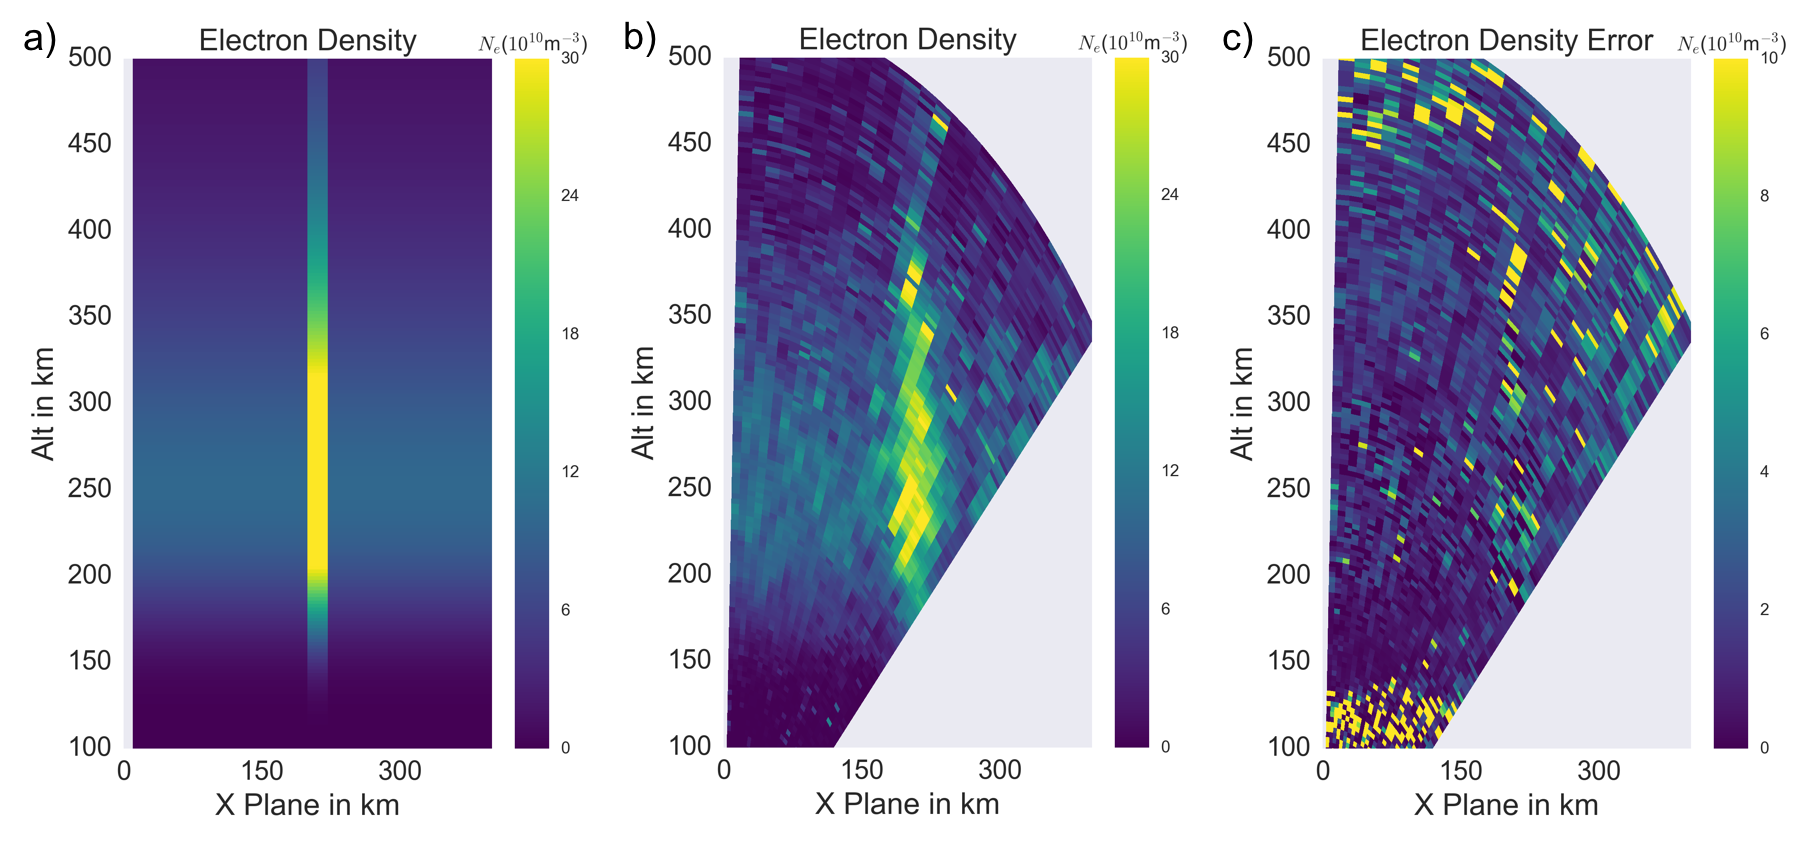
\includegraphics[width=6in]{moving18kminouterr}
\caption{18 km wide enhancement moving simulation at 480 seconds. a) Input $N_e$. a)  b) Fitted $N_e$ with 60 second integration. c) Estimated error from fit.}
\label{fig:moving18all}
\end{figure}

\subsection{Full Parameter Experiment}
Finally, plasma parameters derived from a multi-fluid model developed in \cite{semeter:plasmatransport2012} are used to drive STISRS. The specific example was originally used in \cite{Perry:2015jf} and was designed for comparison to measurements from the Resolute Bay Incoherent Scatter Radar. Images of the plasma parameters can be seen in Figures \ref{fig:plparamst0} and \ref{fig:plparamst60}. These enhancements in electron density, temperature and ion temperature are caused by an auroral arc created from a Region 1 field aligned current system of amplitude .875 $\mu$A/m$^2$, which moves through the field of view at 200 m/s.

\begin{figure}[!t]
\centering
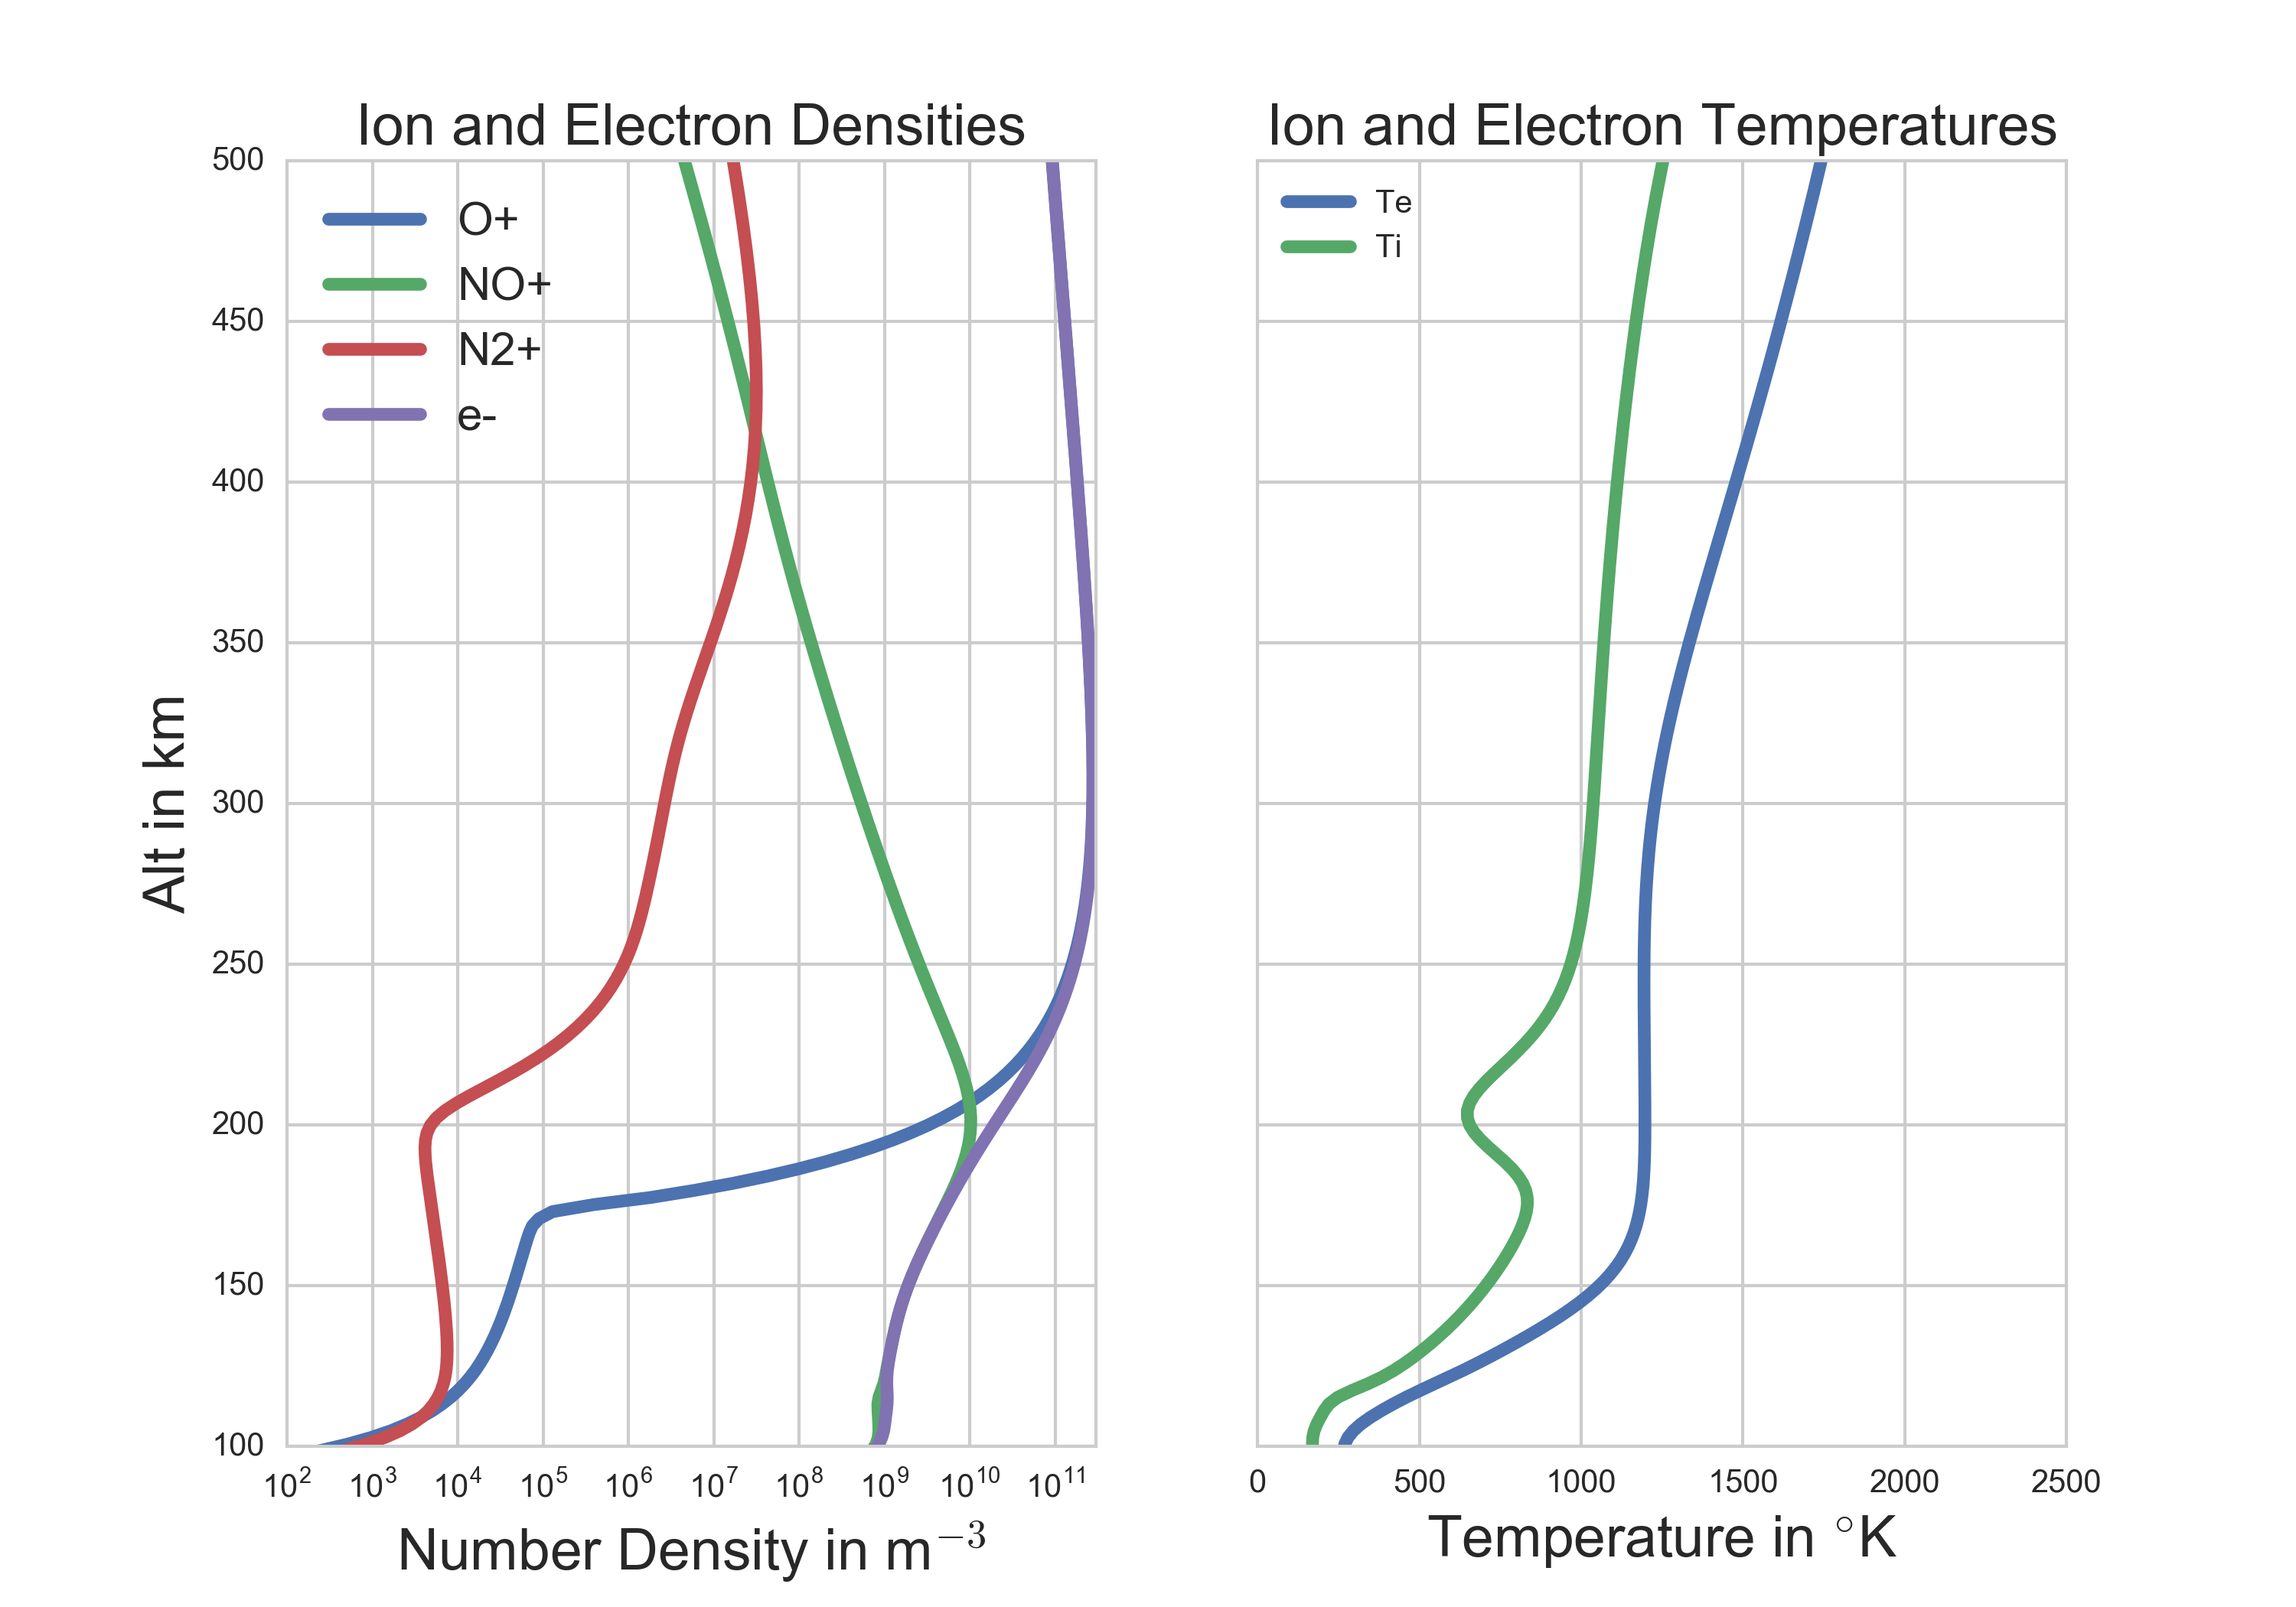
\includegraphics[width=6in]{backgroundallparams}
\caption{Background ionospheric parameters ($N_e$, $T_e$, $T_i$) along with number density of ion species, used for simulations.}
\label{fig:plparamst0}
\end{figure}

\begin{figure}[!t]
\centering
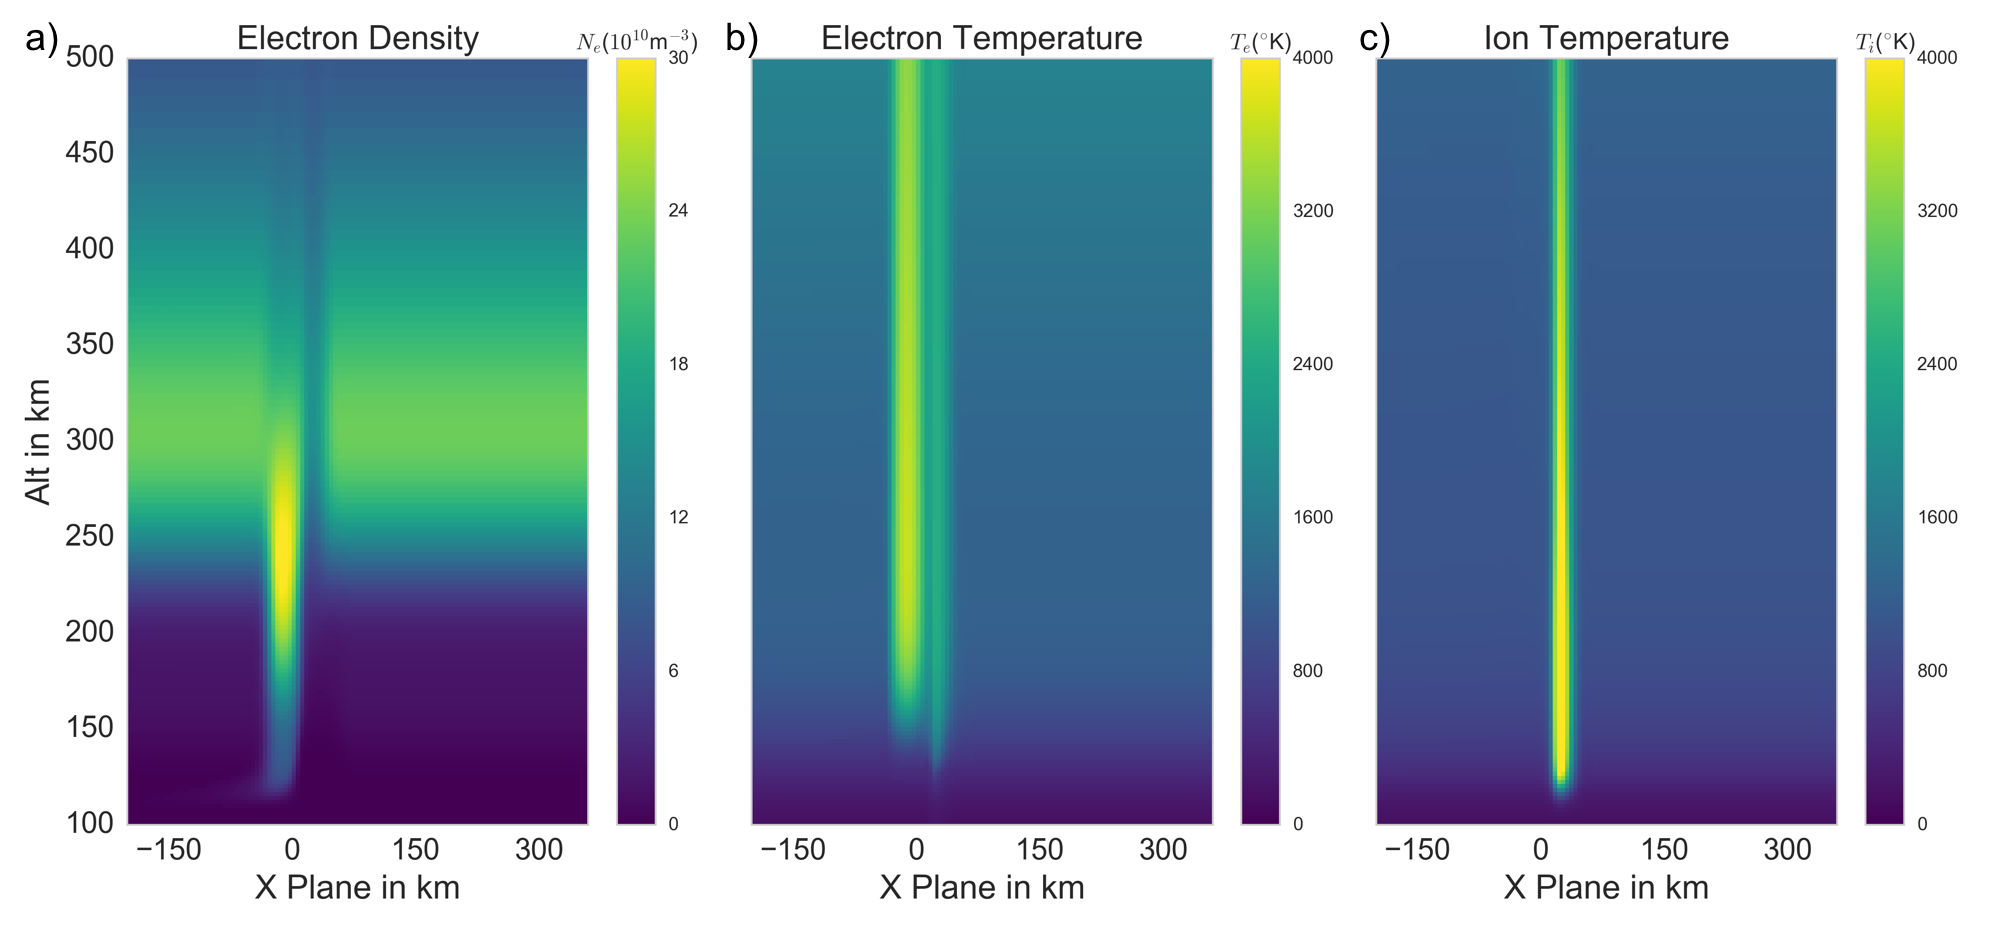
\includegraphics[width=6in]{0960_15_int}
\caption{Perturbations to Figure \ref{fig:plparamst0} due to an imposed current system of .875 $\mu$A/m$^2$ at $t=960$ s, auroral arc.}
\label{fig:plparamst60}
\end{figure}

Using a beam pattern similar to the one seen in the right panel of Figure \ref{fig:background1}, we use STISRS to explore how an electronically scanned ISR may reconstruct the scene. This a best case condition, as we have apriori knowledge of the plane that the arc is traveling in, and have set up the radar spatial beam pattern for the experiment to take advantage of this knowledge. This feature reduces the number of radar beams and required integration time to gain the desired statistics. 

It is also assumed that the ratios between ion species are known. This is a common practice in ISR fitting as allowing the ratios to be free parameters can allow for non-unique solutions depending on the ion species that are present. If the fixed, apriori assumed composition ratios between the different ion species are incorrect, this can lead to errors in the final parameter estimates. For the lower F region ionosphere, generally this usually leads to errors between 150-250 km where the ionosphere changes from NO$^+$ dominated to O$^+$ dominated \cite{Zettergren:2011ej,Blelly:2010gf}. Another aspect from this specific case as the field aligned current passes through this creates an influx of  NO$^+$ in the cross over region for this simulation \cite{Perry:2015jf} .

The output of the STISRS from the parameters can be seen in Figure \ref{fig:fplparamst60}. The integration is started at $t=960$ s into the simulation with the plasma parameters shown in seen in Figure \ref{fig:plparamst60}. For this case, a 60 second integration time is used, which for the 27 beam radar experiment set up gives 255 pulses per position. Lastly the expected errors from the fit can be seen Figure \ref{fig:fplparamst60err}.

We highlight several features in the fitted results. First, enhancements in electron and ion temperature are clearly visible and well above the expected error. Second, we examine whether the cavity in electron density that is formed is also visible. These types of cavities are signs of downward current flow and there has been a question (REF?) as to whether these could be observed well with ISR systems \jcom{awkward-reword}{due to their defining feature being an evacuations of electrons, thus reducing the return power from the scattered signal}. The image in \ref{fig:fplparamst60} shows the best case of finding this cavity with this beam pattern, as at this time the cavity is close to perpendicular with one of the beams. For the other cases where the beams are not well aligned with the cavity it becomes much more difficult to observe it due to the range ambiguity being larger than the beam width, making the "filling in" of the evacuated electrons more pronounced. 

%% Fitted Data

\begin{figure}[!t]
\centering
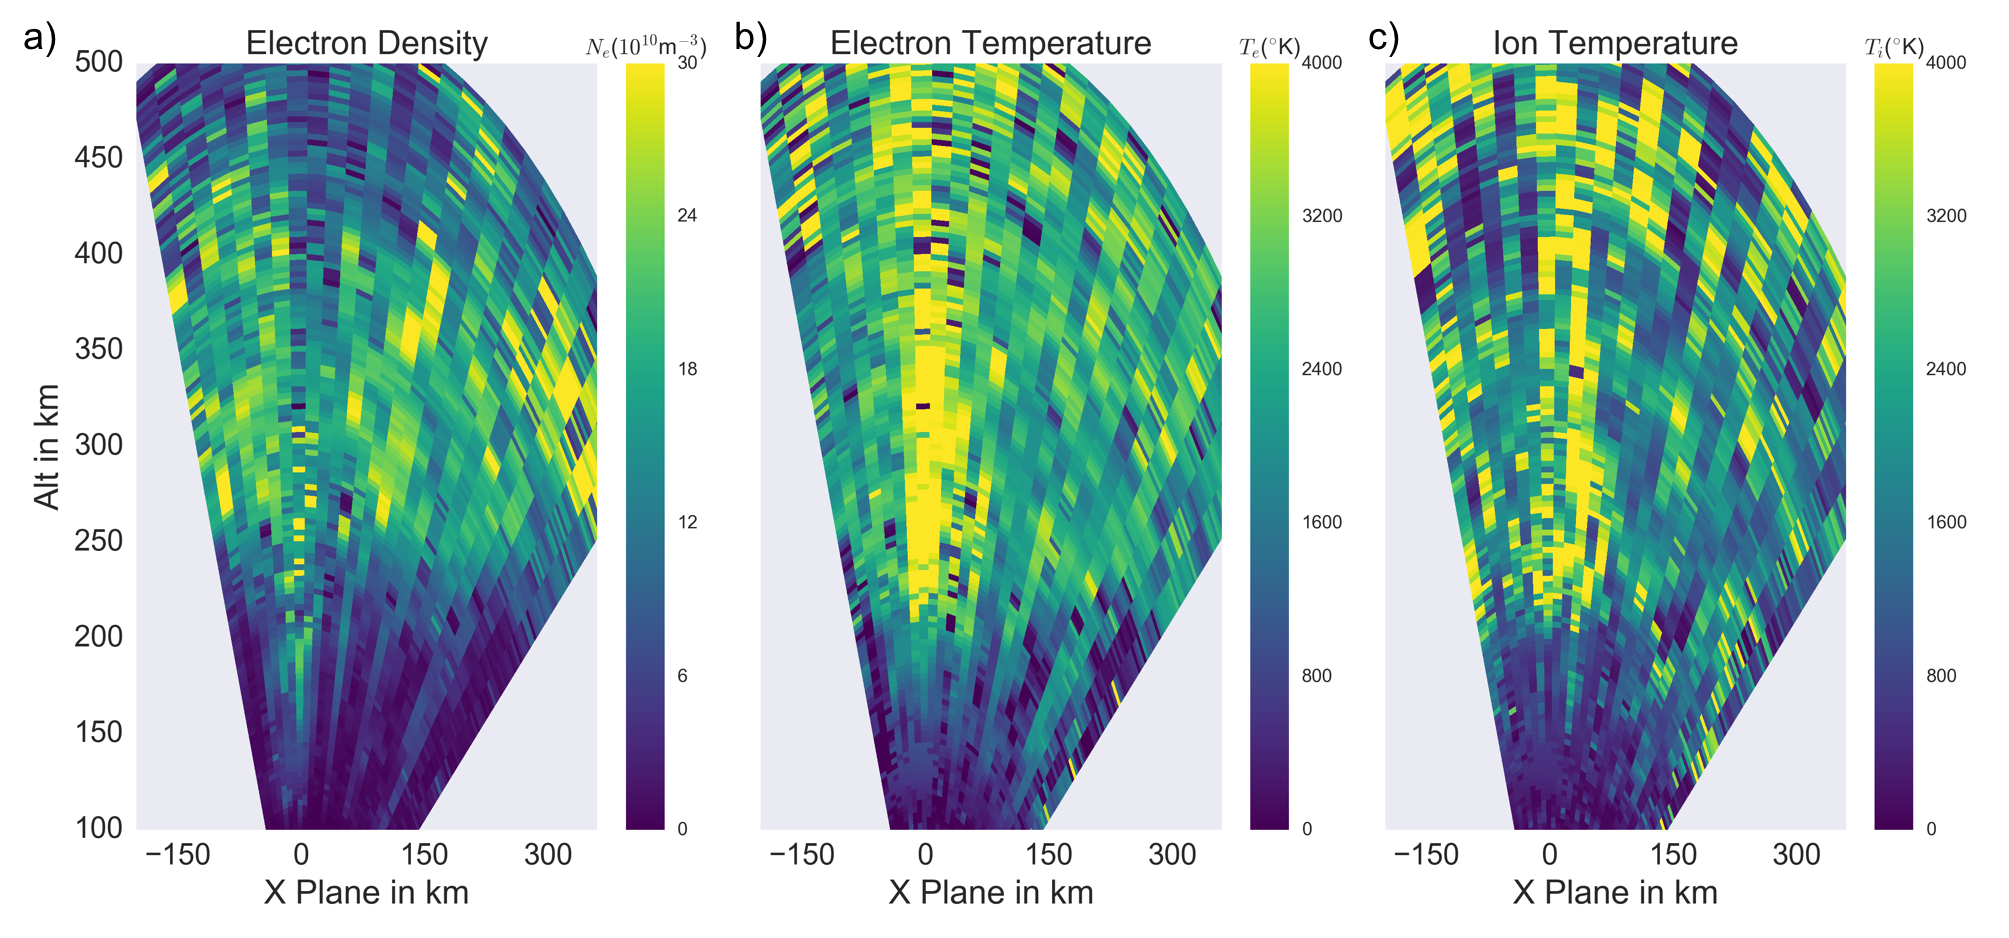
\includegraphics[width=6in]{0960_60_int}
\caption{Fitted Plasma Parameters at $t=960$ s with 60 second integration.}
\label{fig:fplparamst60}
\end{figure}

\begin{figure}[!t]
\centering
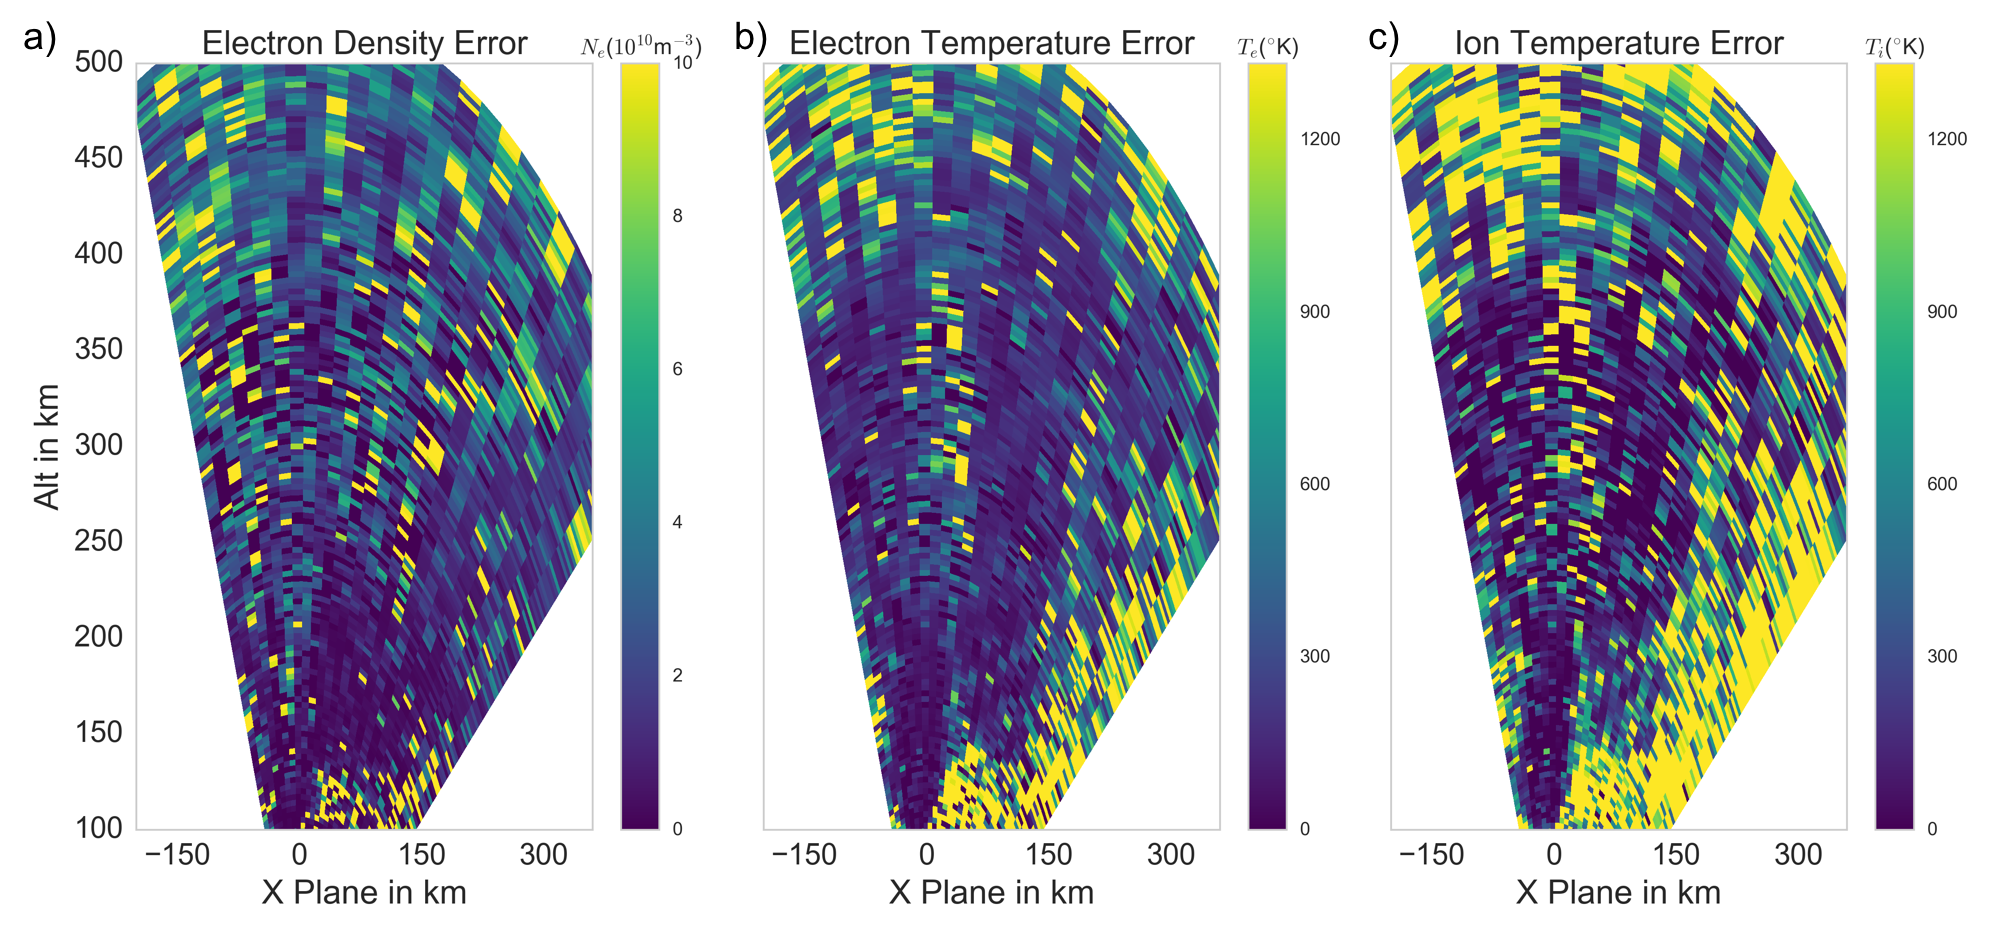
\includegraphics[width=6in]{0960_60_int_err}
\caption{Estimated errors from fitted Plasma Parameters at $t=960$ s with 60 second integration.}
\label{fig:fplparamst60err}
\end{figure}

